\chapter{Results} \label{ch:results}
% \section{Metric Based Analysis}
% \section{Visual Based Analysis}
In line with the research questions, the evaluation section aims to quantify the performance gains obtained by using the Proxy Attention method. The section will compare the performance of networks that were trained with, and without Proxy Attention on the basis of classification metrics, and explainability improvements.

Note that complete performance logs can be found in the appendix.
\section{Accuracy}
This section explores the validation accuracy obtained by the models for different hyperparameters and datasets. Since the task at hand is a classification task, this measure is a direct comparison of the performance of the models.

\subsection{Results Per Dataset}
This subsection shows the accuracies per model for each dataset. Tabulated results can be found in the appendix.

\subsection{Tsinghua Dogs and Places256 Results}
This section shows the accuracies per model for the Tsinghua Dogs and Places256 datasets. The results are shown in Figure \ref{fig:tsing_places256_results}.

\begin{figure}[H]
    % \centering
    \begin{subfigure}[h]{.5\textwidth}
        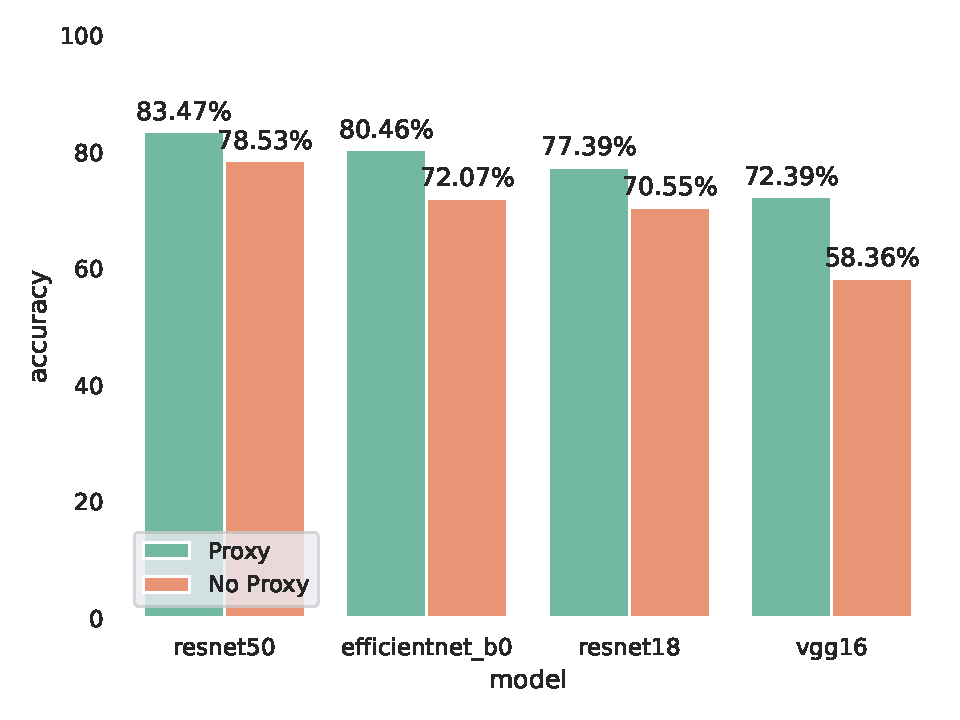
\includegraphics[width=\linewidth, right]{results/tsing_results.pdf}
        \caption{Tsinghua Dogs Dataset}
    \end{subfigure}
    % \hfill
    \begin{subfigure}[h]{.5\textwidth}
        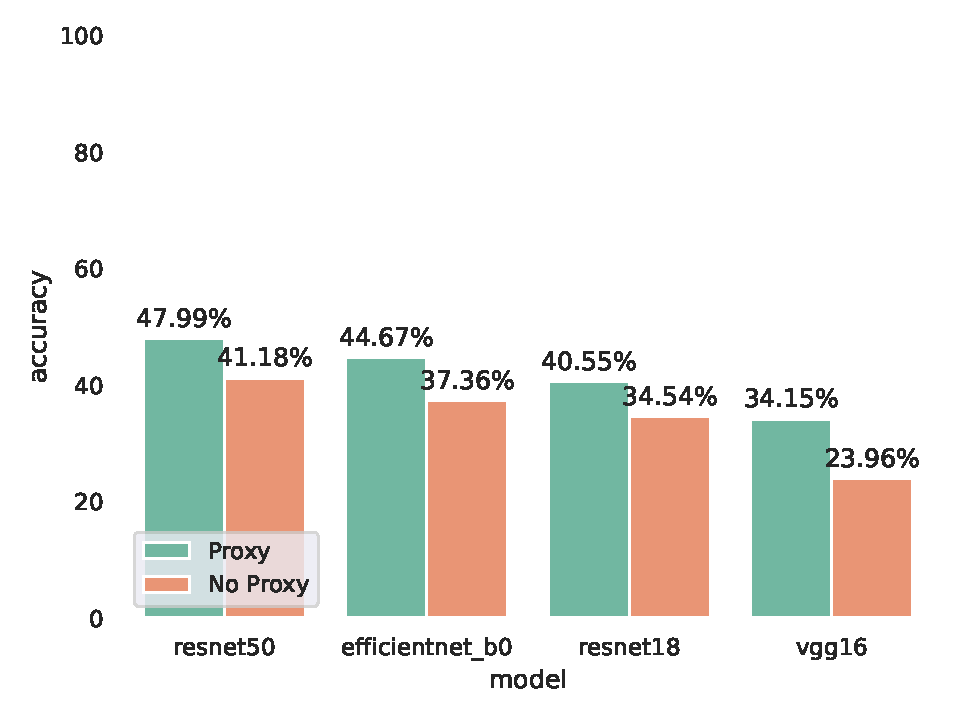
\includegraphics[width=\linewidth, left]{results/places256_results.pdf}
        \caption{Places256 Dataset}
    \end{subfigure}
    \caption{Comparing Accuracies of models trained with and without Proxy Attention on the Tsinghua Dogs and Places256 datasets}
    \label{fig:tsing_places256_results}
\end{figure}

\subsection{Stanford Dogs and Cifar100 Results}
This section shows the accuracies per model for the Stanford Dogs and Cifar100 datasets. The results are shown in Figure \ref{fig:dogs_cifar100_results}.
\begin{figure}[H]
    % \centering
    \begin{subfigure}[h]{.5\textwidth}
        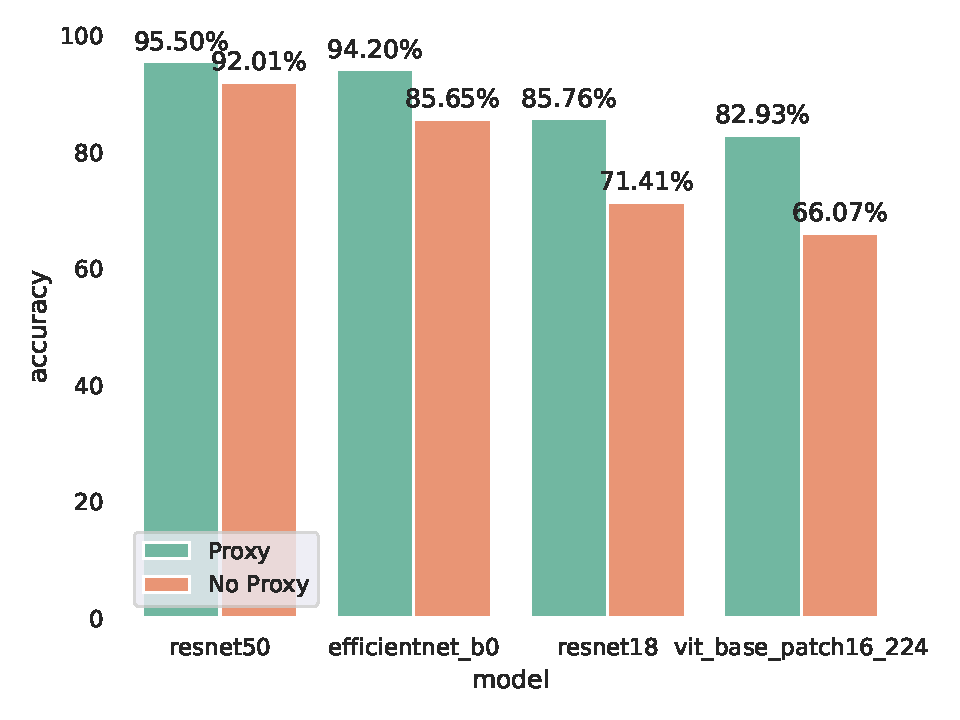
\includegraphics[width=\linewidth, right]{results/dogs_results.pdf}
        \caption{Stanford Dogs Dataset}
    \end{subfigure}
    % \hfill
    \begin{subfigure}[h]{.5\textwidth}
        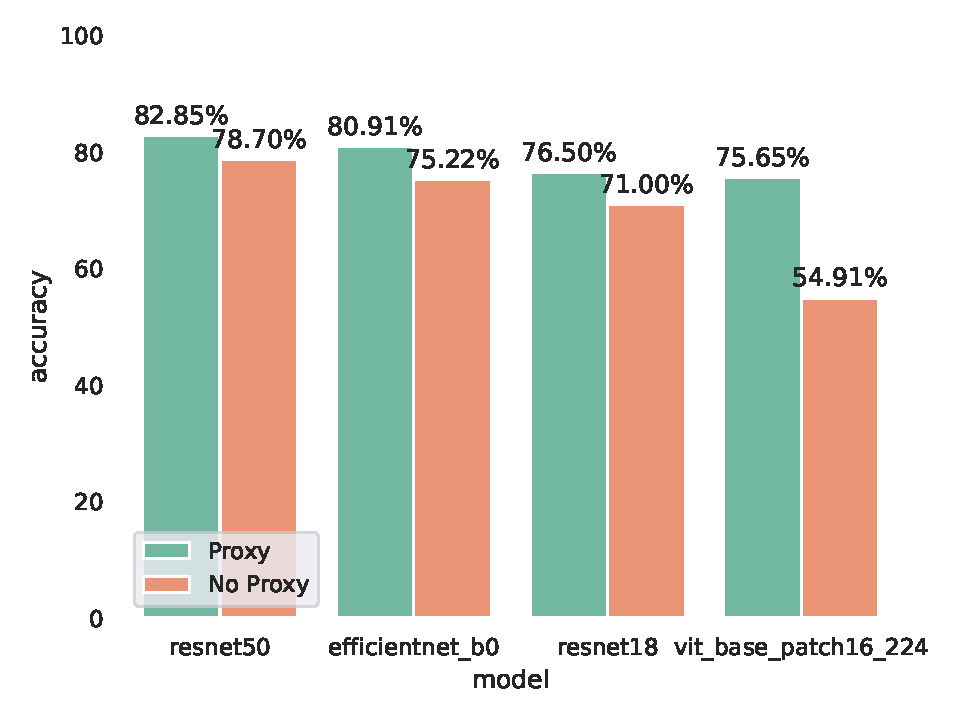
\includegraphics[width=\linewidth, left]{results/cifar100_results.pdf}
        \caption{Cifar100 Dataset}
    \end{subfigure}
    \caption{Comparing Accuracies of models trained with and without Proxy Attention on the Stanford Dogs and Cifar100 datasets}
    \label{fig:dogs_cifar100_results}
\end{figure}

\subsection{Caltech101 and Asl Results}
This section shows the accuracies per model for the Caltech101 and Asl datasets. The results are shown in Figure \ref{fig:caltech101_asl_results}.
\begin{figure}[H]
    % \centering
    \begin{subfigure}[h]{.5\textwidth}
        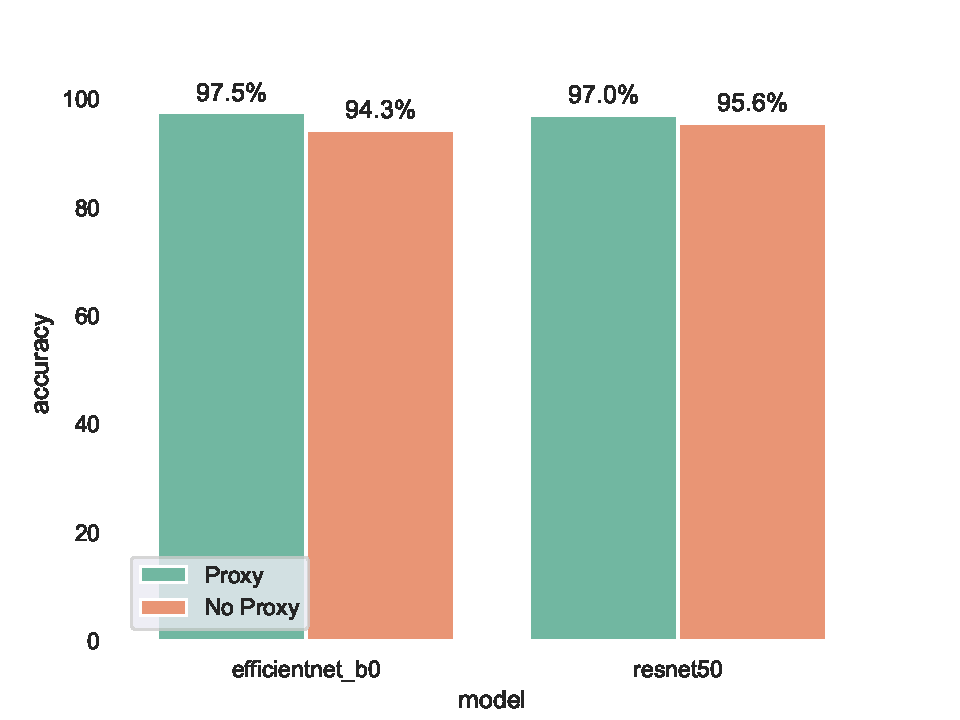
\includegraphics[width=\linewidth, right]{results/caltech101_results.pdf}
        \caption{Caltech101 Dataset}
    \end{subfigure}
    % \hfill
    \begin{subfigure}[h]{.5\textwidth}
        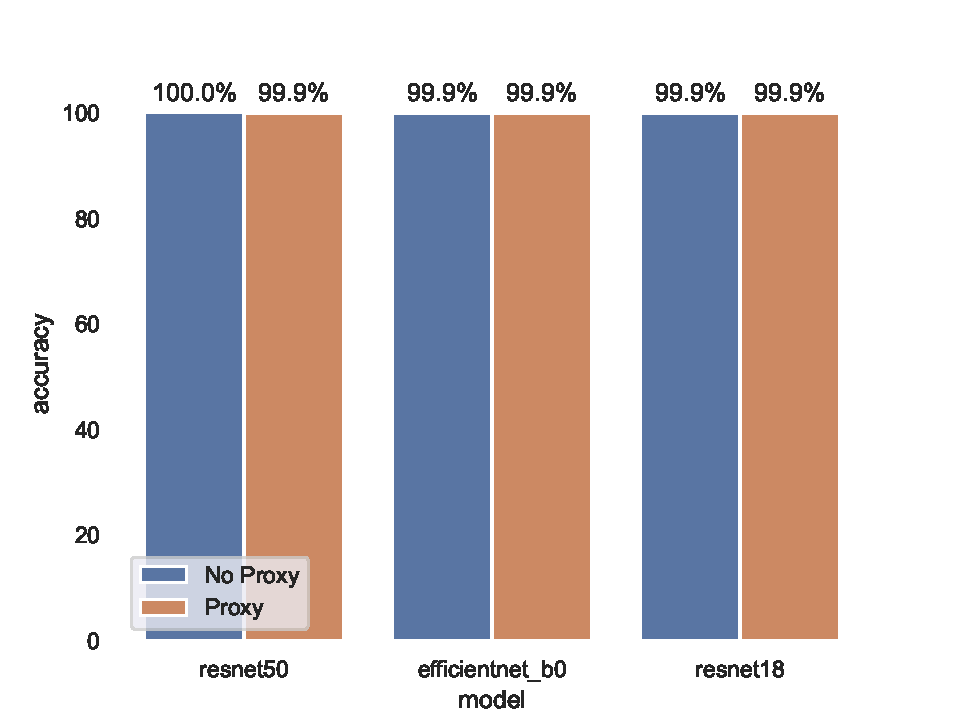
\includegraphics[width=\linewidth, left]{results/asl_results.pdf}
        \caption{Asl Dataset}
    \end{subfigure}
    \caption{Comparing Accuracies of models trained with and without Proxy Attention on the Caltech101 and Asl datasets}
    \label{fig:caltech101_asl_results}
\end{figure}

\subsection{Plantdisease Results}
This section shows the accuracies per model for the Plantdisease dataset. The results are shown in Figure \ref{fig:plantdisease_results}. 
\begin{figure}[H]
    \centering
    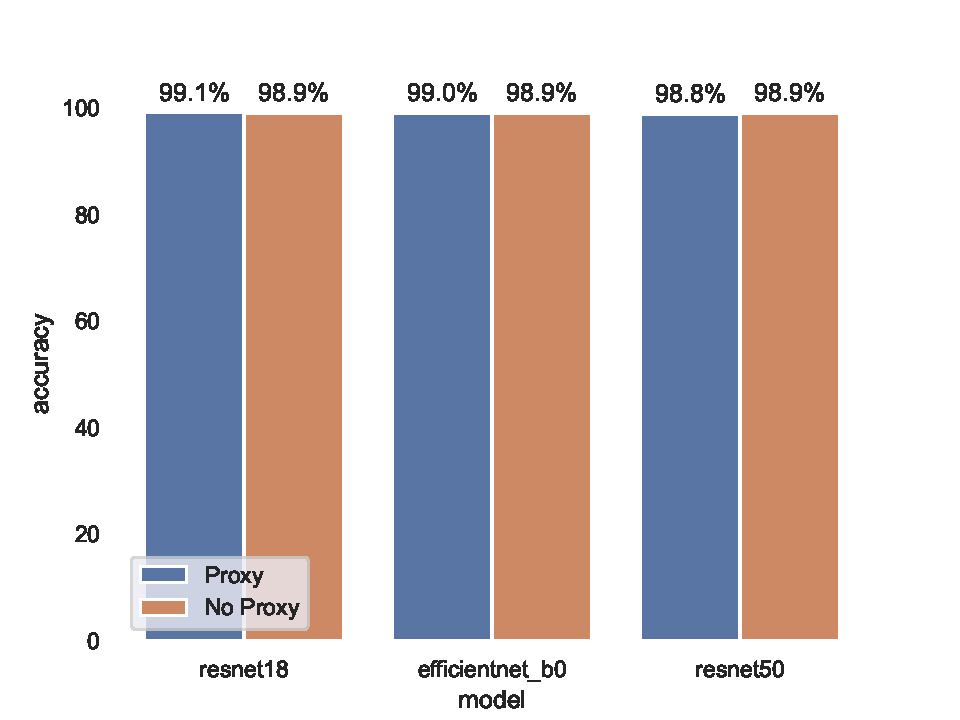
\includegraphics[width=.6\linewidth]{results/plantdisease_results.pdf}
    \caption{Comparing Accuracies of models trained with and without Proxy Attention on the Plantdisease dataset}
    \label{fig:plantdisease_results}
\end{figure}


\subsection{Results Grouped By Schedule}
This section explores the validation accuracy obtained for different step schedules. The results are shown in Figure \ref{fig:schedresnet50_results}. 
\begin{figure}[H]
    \centering
    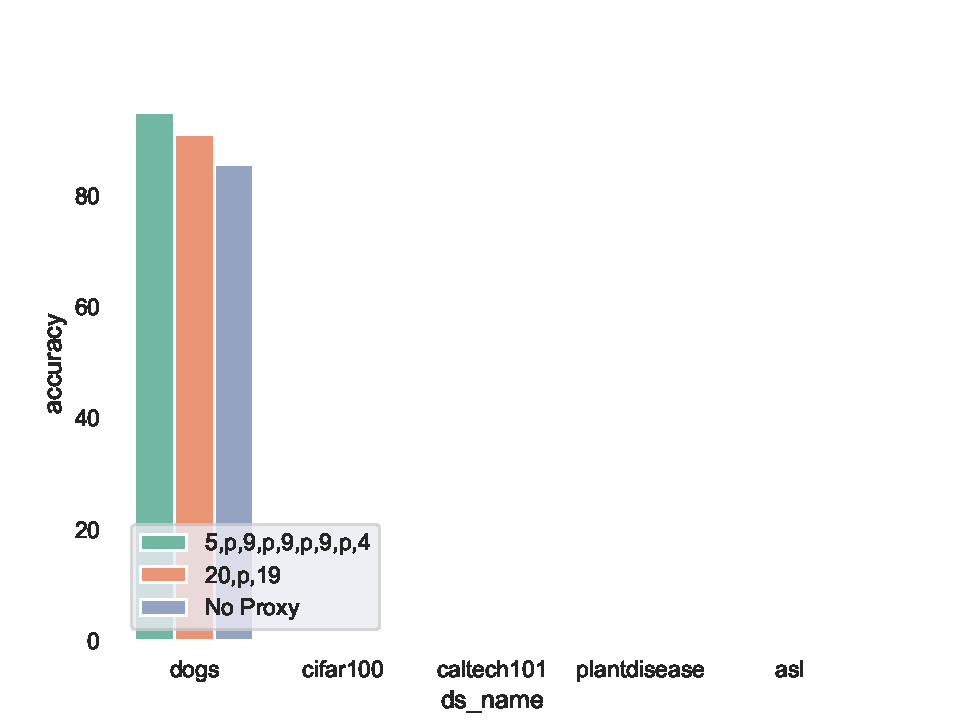
\includegraphics[width=.6\textwidth]{results/schedule_resnet50.pdf}
    \caption{Comparing Accuracies of models trained with and without Proxy Attention on the ResNet50 \cite{heDeepResidualLearning2016} architecture for different step schedules}.
    \label{fig:schedresnet50_results}
\end{figure}

\subsection{Results Grouped By Proxy Threshold}
This section explores the validation accuracy obtained for different Proxy thresholds. The results are shown in Figure \ref{fig:proxy_threshold}. 
\begin{figure}[H]
    \begin{subfigure}[h]{.5\textwidth}
        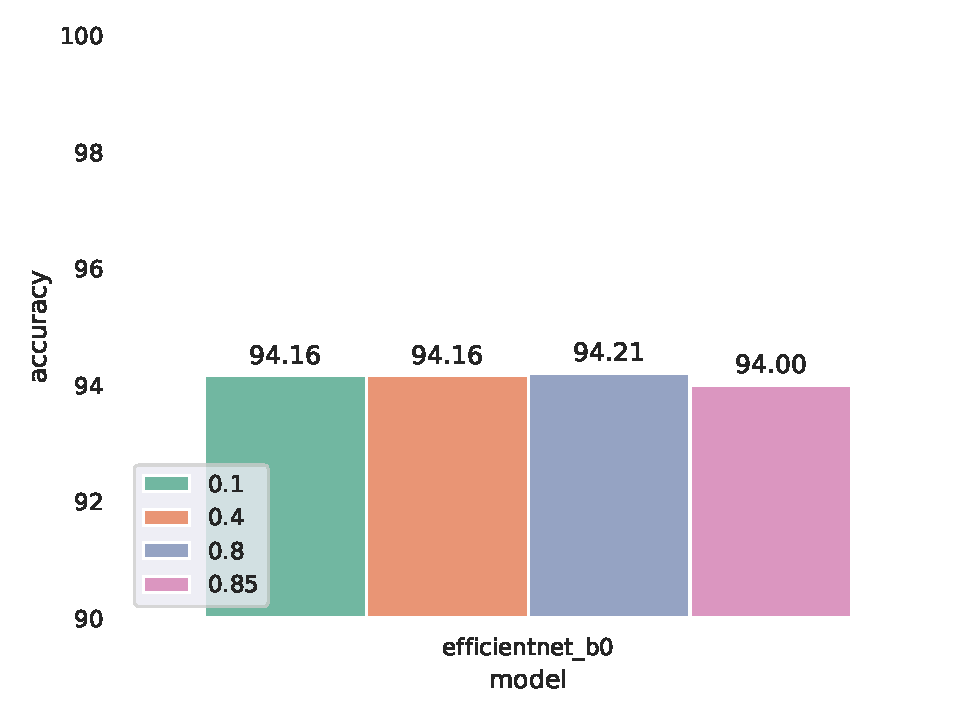
\includegraphics[width=\linewidth, right]{results/proxy_threshold_results.pdf}
        \caption{EfficientNetB0 \cite{tanEfficientnetRethinkingModel2019} trained with Proxy Attention on the Stanford Dogs dataset\cite{khoslaNovelDatasetFineGrained}}
    \end{subfigure}
    % \hfill
    \begin{subfigure}[h]{.5\textwidth}
        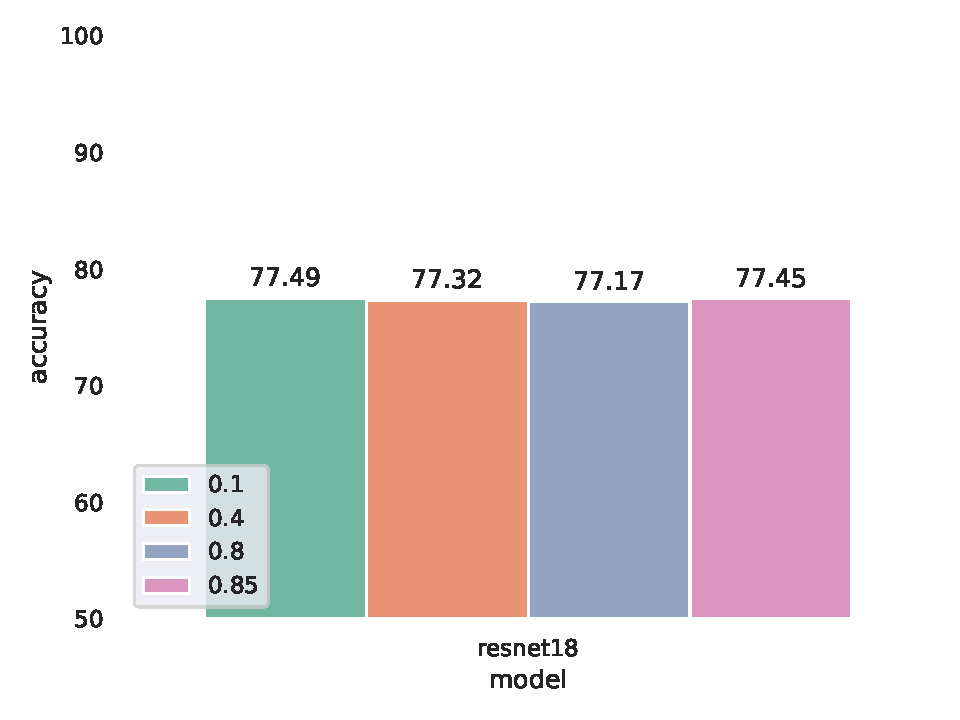
\includegraphics[width=\linewidth, left]{results/proxy_threshold_results_tsing.pdf}
        \caption{Resnet18 \cite{heDeepResidualLearning2016} trained with Proxy Attention on the Tsinghua Dogs Dataset \cite{zouNewDatasetDog2020}}
    \end{subfigure}
    
    \caption{Comparing Accuracies of models trained with Proxy Attention for different Proxy Thresholds}
    \label{fig:proxy_threshold}
\end{figure}

\subsection{Results Grouped By Proxy Image Weight}
This section explores the validation accuracy obtained for different Proxy image weights. The results are shown in Figure \ref{fig:proxy_weight}. 

% \begin{figure}[H]
%     \centering
%     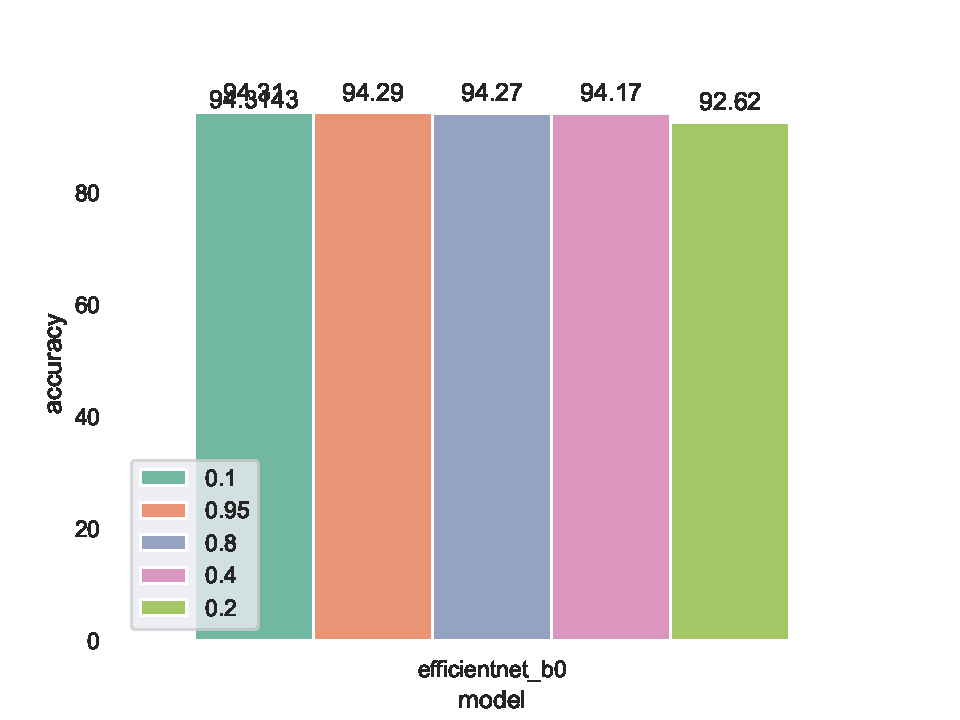
\includegraphics[width=1\textwidth]{results/proxy_weight_results.pdf}
%     \caption{Comparing Accuracies of EfficientNetB0 \cite{tanEfficientnetRethinkingModel2019} trained with Proxy Attention on the Stanford Dogs dataset\cite{khoslaNovelDatasetFineGrained} for different Proxy Image Weights}
%     \label{fig:proxy_weight}
% \end{figure}

% \begin{figure}[H]
%     \centering
%     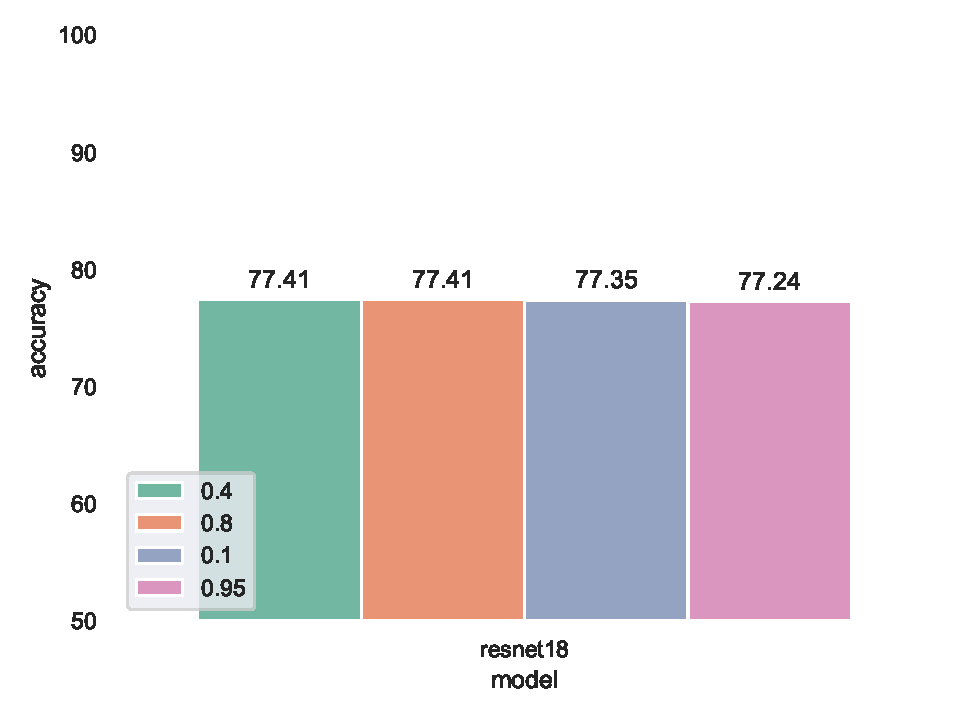
\includegraphics[width=1\textwidth]{results/proxy_weight_results_tsing.pdf}
%     \caption{Comparing Accuracies of Resnet18 \cite{heDeepResidualLearning2016} trained with Proxy Attention on the Tsinghua Dogs Dataset \cite{zouNewDatasetDog2020} for different Proxy Image Weights}
%     \label{fig:proxy_weight2}
% \end{figure}

\begin{figure}[H]
    \begin{subfigure}[h]{.5\textwidth}
        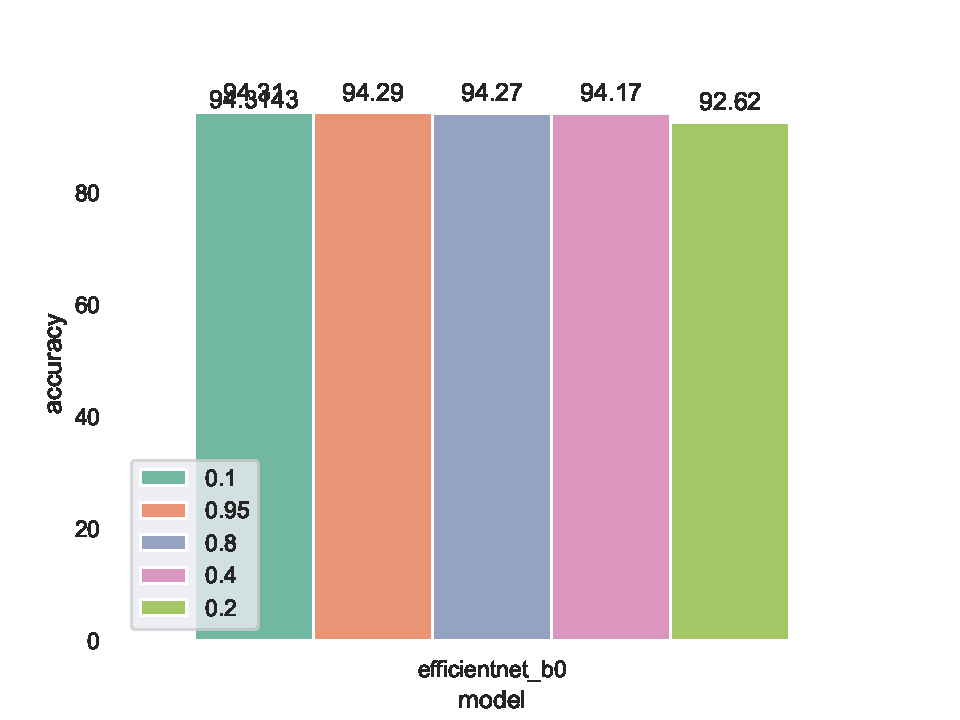
\includegraphics[width=\linewidth, right]{results/proxy_weight_results.pdf}
        \caption{EfficientNetB0 \cite{tanEfficientnetRethinkingModel2019} trained with Proxy Attention on the Stanford Dogs dataset\cite{khoslaNovelDatasetFineGrained}}
    \end{subfigure}
    % \hfill
    \begin{subfigure}[h]{.5\textwidth}
        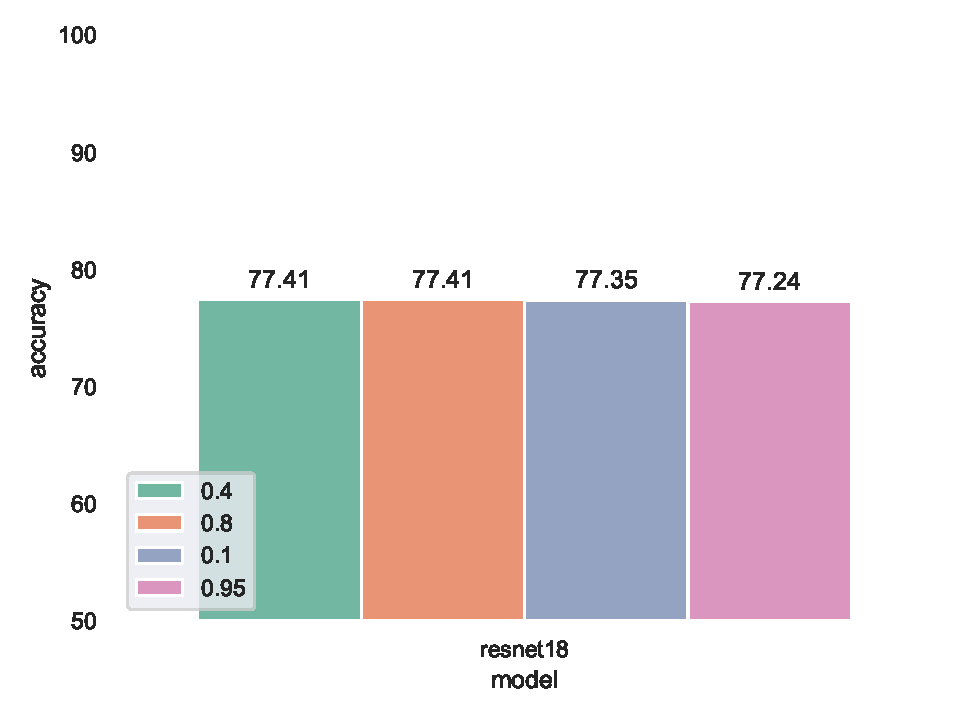
\includegraphics[width=\linewidth, left]{results/proxy_weight_results_tsing.pdf}
        \caption{Resnet18 \cite{heDeepResidualLearning2016} trained with Proxy Attention on the Tsinghua Dogs Dataset \cite{zouNewDatasetDog2020}}
    \end{subfigure}
    
    \caption{Comparing Accuracies of models trained with Proxy Attention for different Proxy Image Weights}
    \label{fig:proxy_weight}
\end{figure}

\subsection{Results Grouped By Proxy Image Subset}
This section explores the validation accuracy obtained for different Proxy image subsets. The results are shown in Figure \ref{fig:proxy_subset}.

% \begin{figure}[H]
%     \centering
%     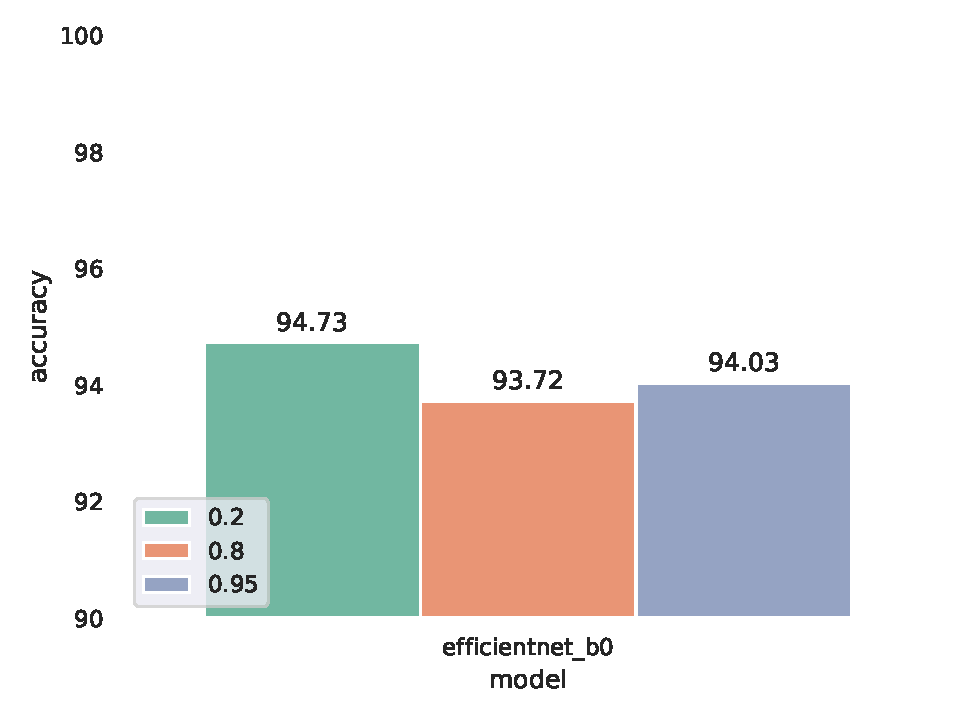
\includegraphics[width=1\textwidth]{results/proxy_subset_attention_results.pdf}
%     \caption{Comparing Accuracies of EfficientNetB0 \cite{tanEfficientnetRethinkingModel2019} trained with Proxy Attention on the Stanford Dogs dataset\cite{khoslaNovelDatasetFineGrained} for different Proxy Image Subsets}
%     \label{fig:proxy_subset}
% \end{figure}

% \begin{figure}[H]
%     \centering
%     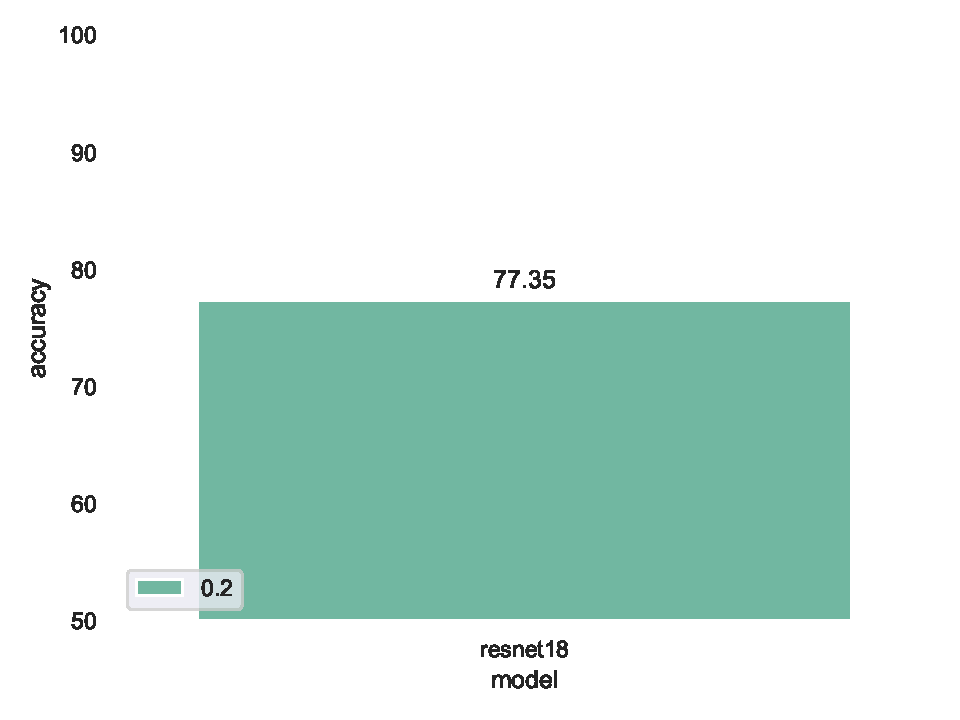
\includegraphics[width=1\textwidth]{results/proxy_subset_results_tsing.pdf}
%     \caption{Comparing Accuracies of Resnet18 \cite{heDeepResidualLearning2016} trained with Proxy Attention on the Tsinghua Dogs Dataset \cite{zouNewDatasetDog2020} for different Proxy Image Subsets}
%     \label{fig:proxy_subset2}
% \end{figure}

\begin{figure}[H]
    \begin{subfigure}[h]{.5\textwidth}
        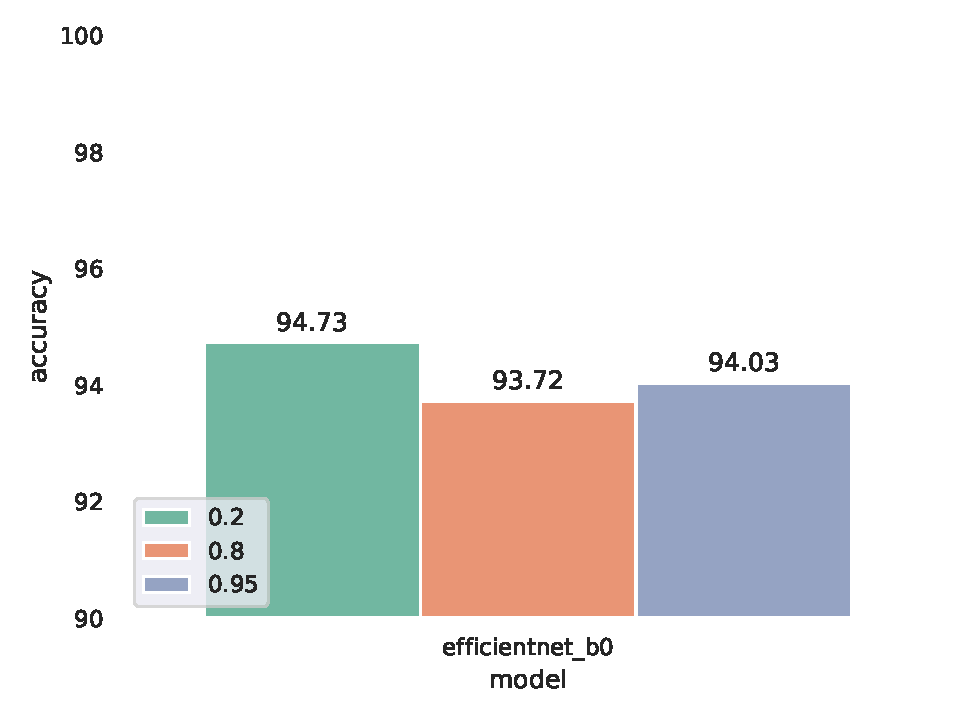
\includegraphics[width=\linewidth, right]{results/proxy_subset_attention_results.pdf}
        \caption{EfficientNetB0 \cite{tanEfficientnetRethinkingModel2019} trained with Proxy Attention on the Stanford Dogs dataset\cite{khoslaNovelDatasetFineGrained}}
    \end{subfigure}
    % \hfill
    \begin{subfigure}[h]{.5\textwidth}
        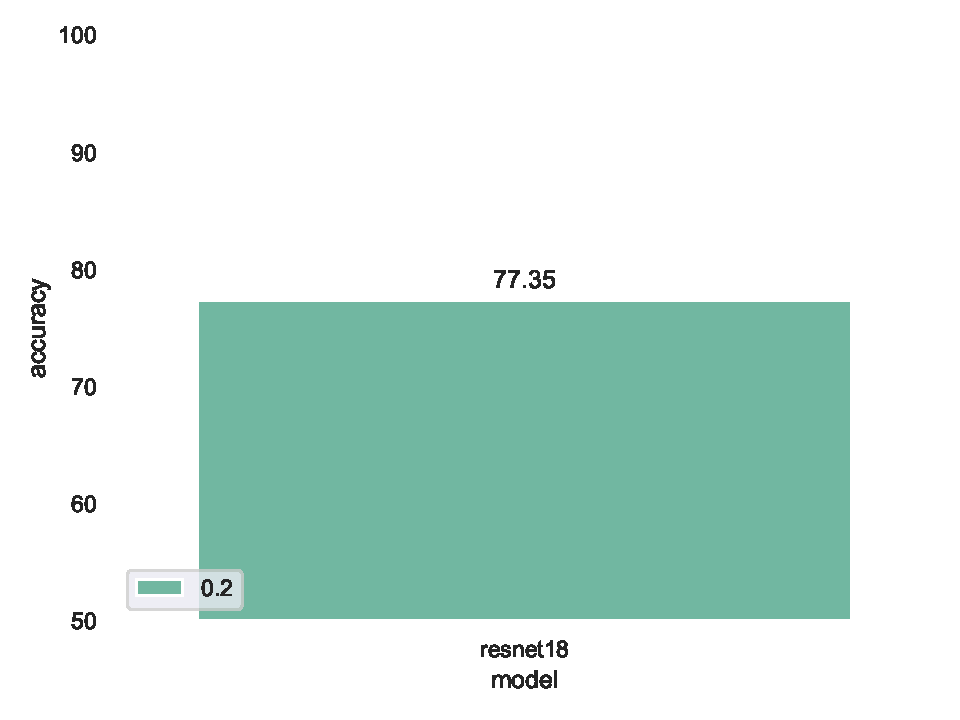
\includegraphics[width=\linewidth, left]{results/proxy_subset_results_tsing.pdf}
        \caption{Resnet18 \cite{heDeepResidualLearning2016} trained with Proxy Attention on the Tsinghua Dogs Dataset \cite{zouNewDatasetDog2020}}
    \end{subfigure}
    
    \caption{Comparing Accuracies of models trained with Proxy Attention for different Proxy Image Subsets}
    \label{fig:proxy_subset}
\end{figure}

\section{Explanability}
This section explores the explainability of the models for different hyperparameters and datasets by using a trained model to generate attention maps for a given input image. The attention maps are compared between the same network (with the same hyperparameters) trained with and without Proxy Attention.

\subsection{CIFAR 100, ResNet18, EigenGradCAM}
\begin{figure}[H]
    \begin{subfigure}[b]{1\textwidth}
        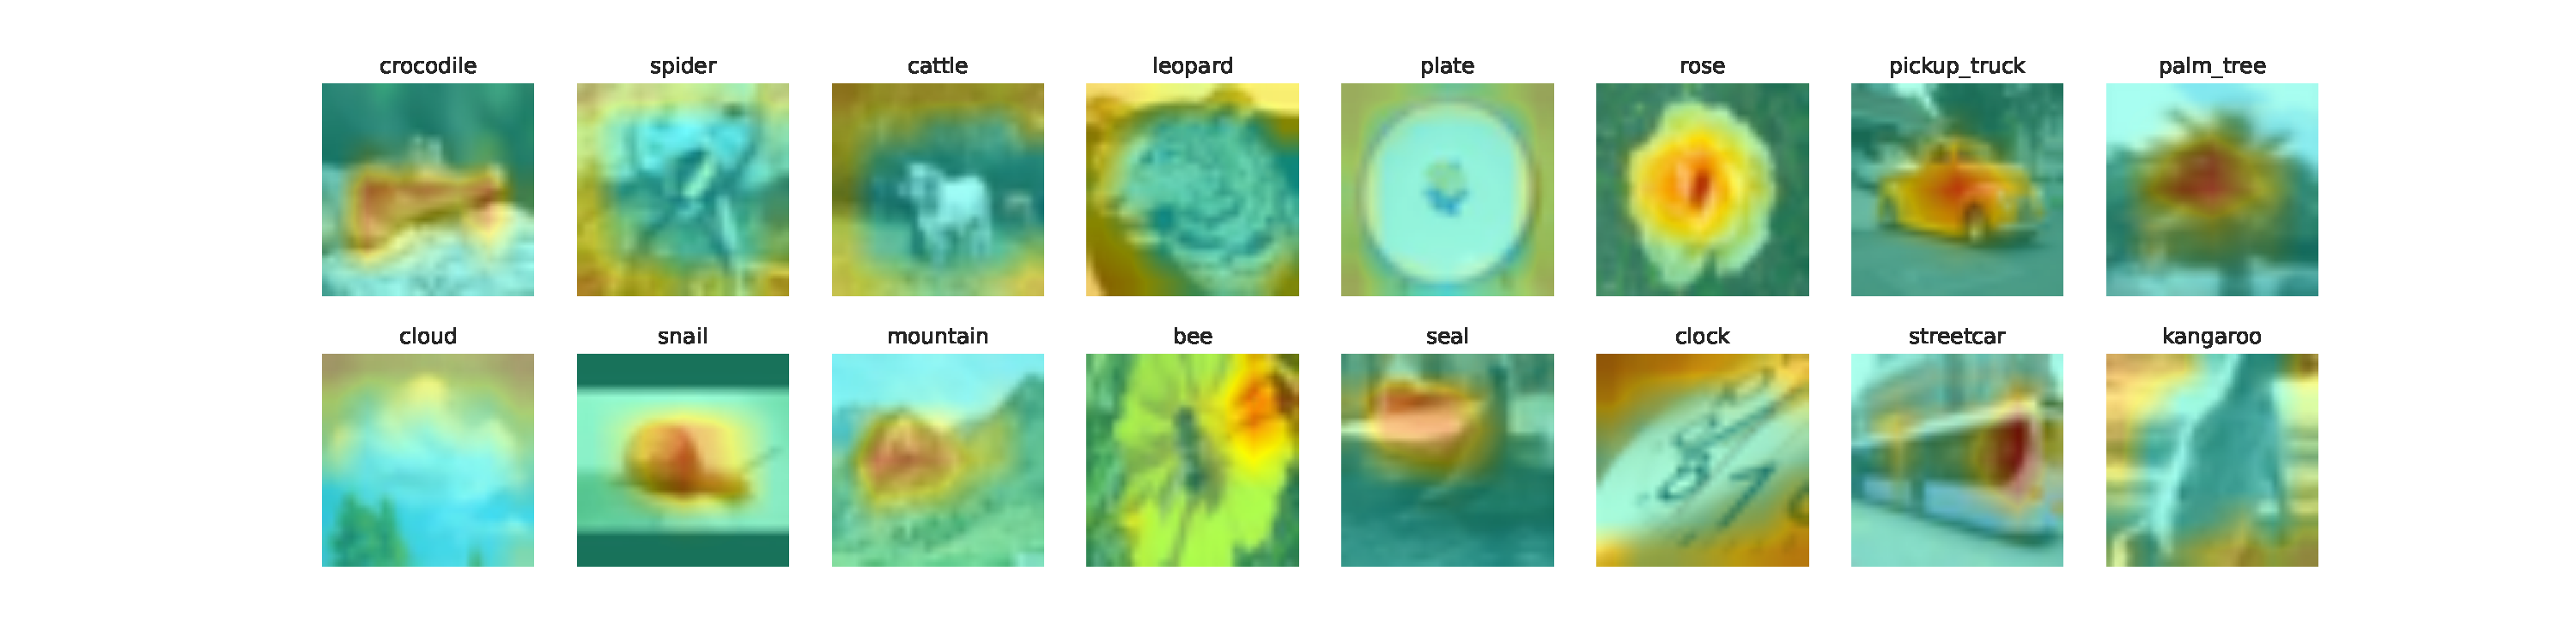
\includegraphics[width=\linewidth]{images/cifar100_resnet18_noproxy_0.pdf}
        \caption{Without Proxy Attention}
    \end{subfigure}
    \begin{subfigure}[b]{1\textwidth}
        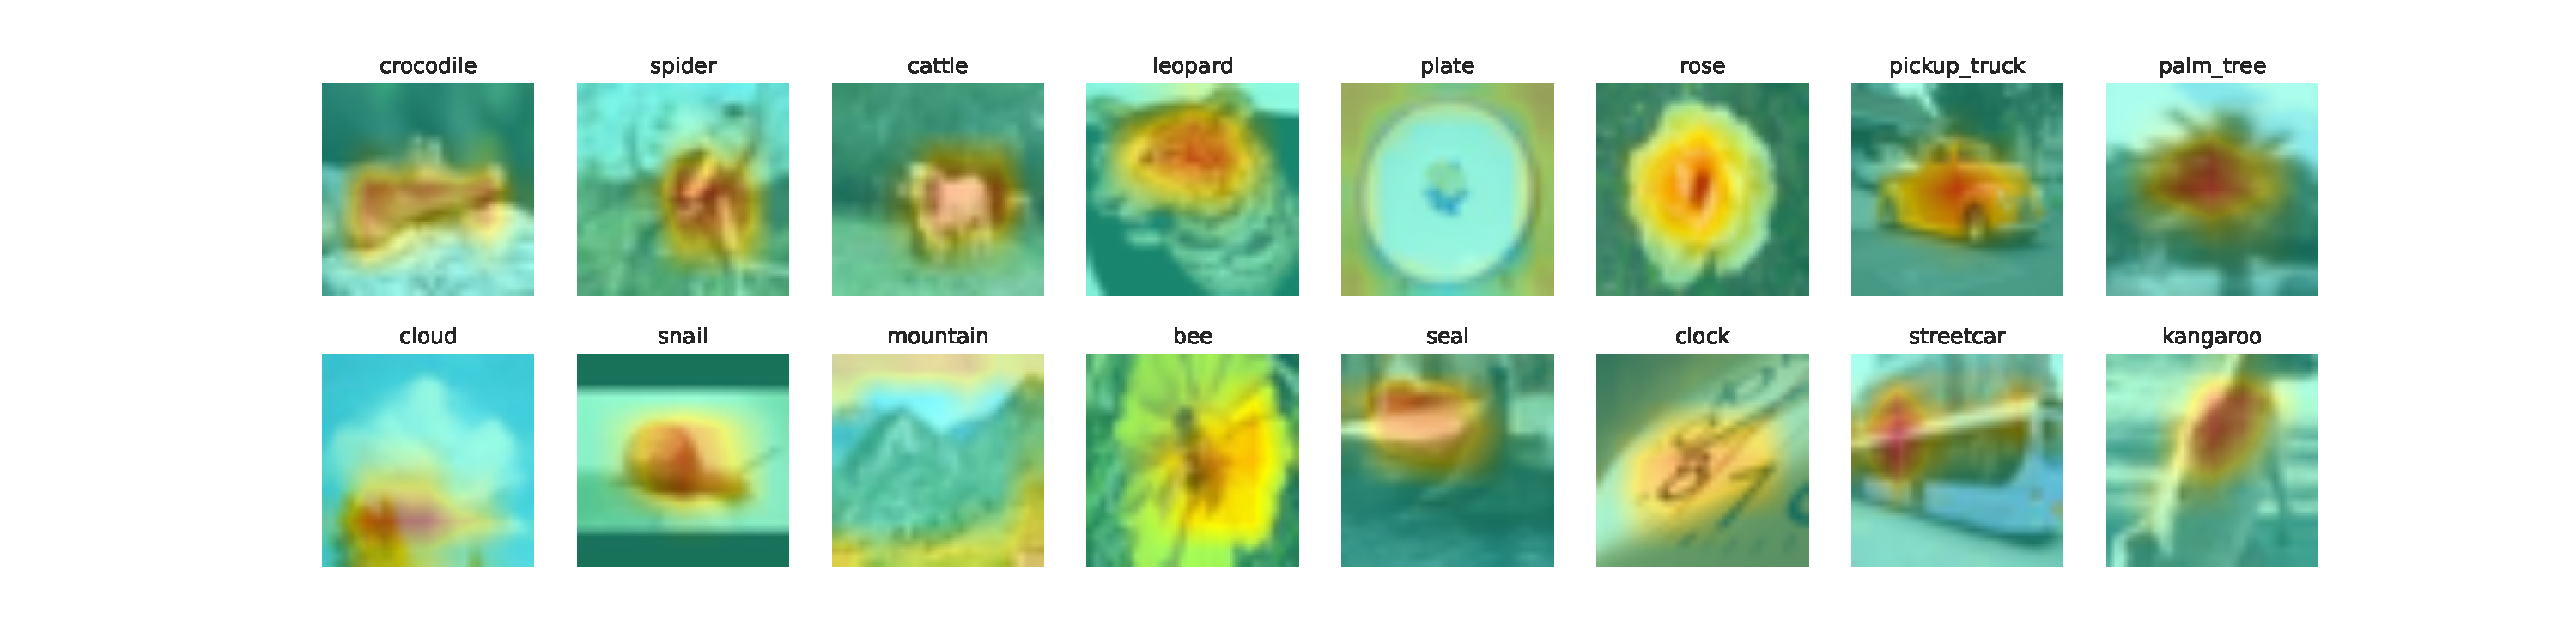
\includegraphics[width=\linewidth]{images/cifar100_resnet18_proxy_0.pdf}
        \caption{With Proxy Attention}
    \end{subfigure}
    
    \caption{Comparison of attention maps generated by resnet18 trained with and without Proxy Attention on the cifar100 dataset}
    \label{fig:resnet18_cifar100}
\end{figure}


\subsection{CIFAR 100, EfficientNetB0, EigenGradCAM}
\begin{figure}[H]
    \begin{subfigure}[b]{1\textwidth}
        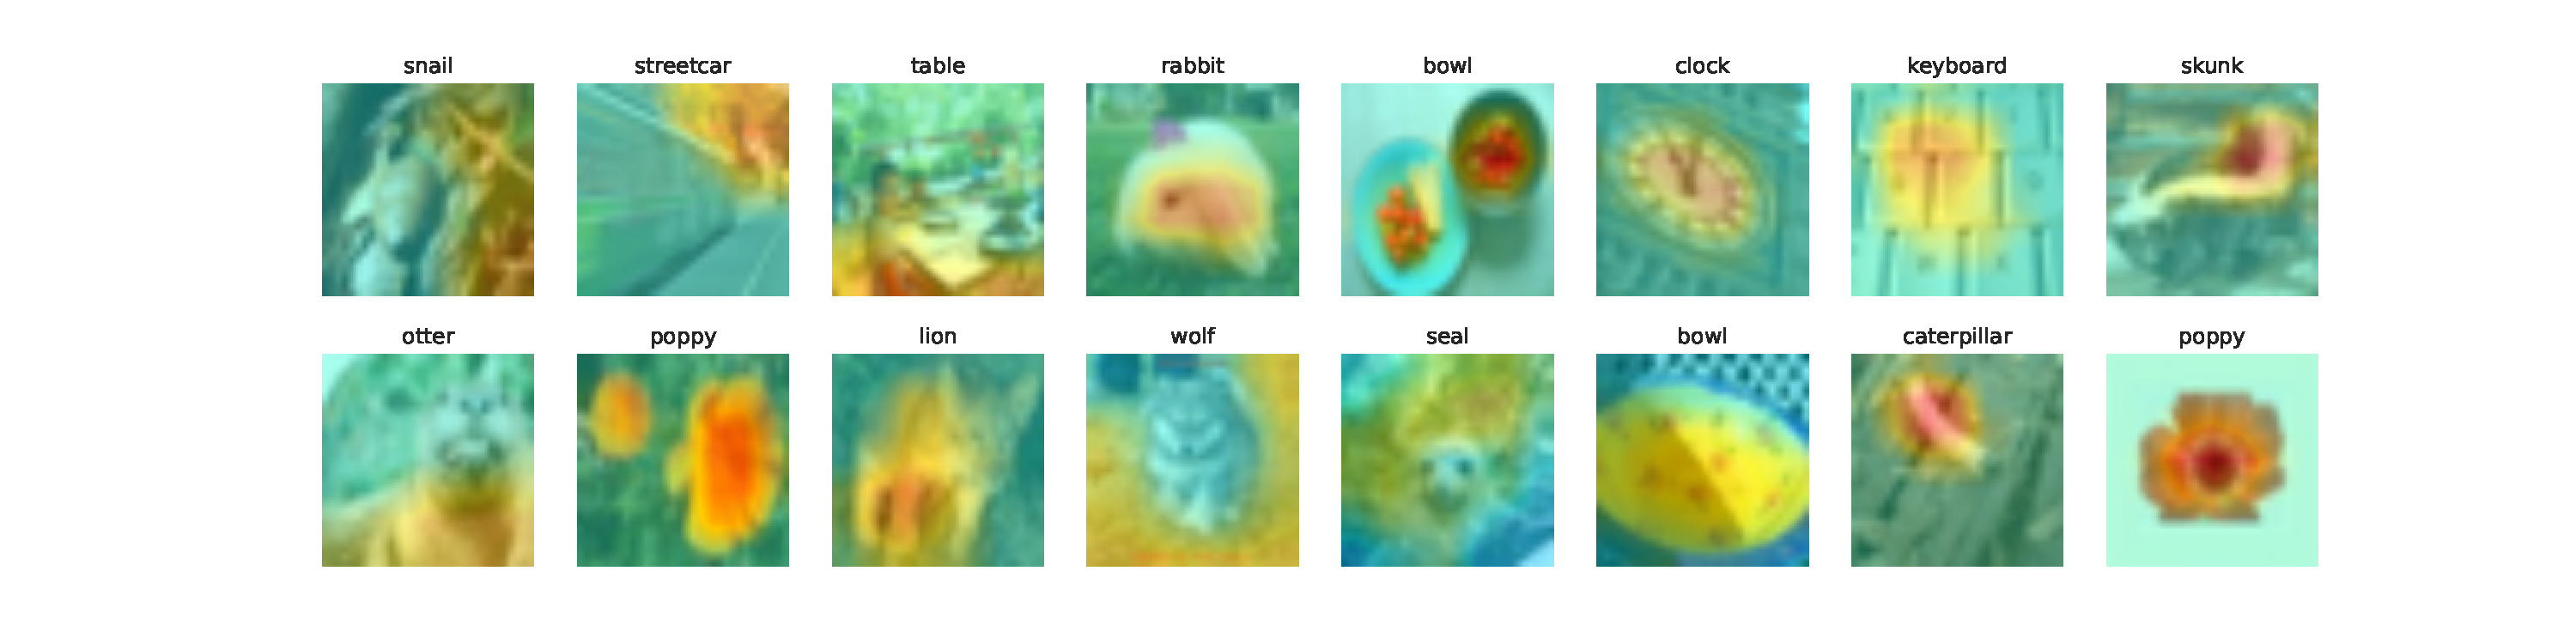
\includegraphics[width=\linewidth]{images/cifar100_efficientnet_b0_noproxy_0.pdf}
        \caption{Without Proxy Attention}
    \end{subfigure}
    \begin{subfigure}[b]{1\textwidth}
        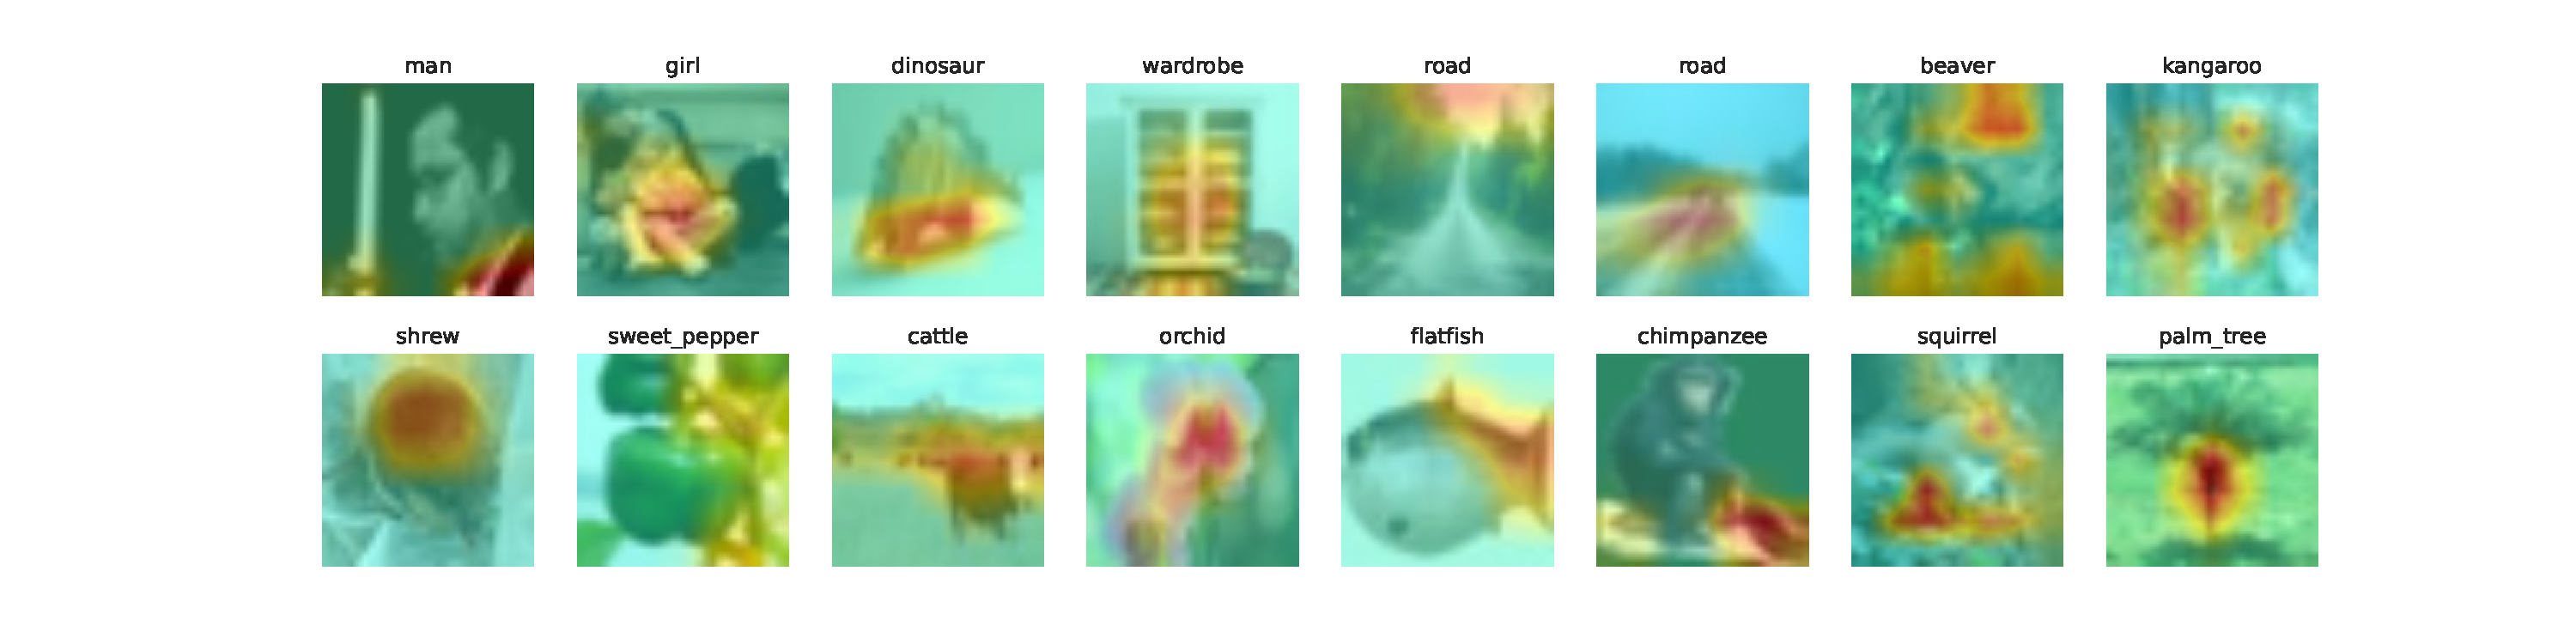
\includegraphics[width=\linewidth]{images/cifar100_efficientnet_b0_proxy_0.pdf}
        \caption{With Proxy Attention}
    \end{subfigure}

    \caption{Comparison of attention maps generated by efficientnet\_b0 trained with and without Proxy Attention on the cifar100 dataset}
    \label{fig:efficientnet_b0_cifar100}
\end{figure}
    


\subsection{CIFAR 100, ViT , EigenGradCAM}
% 
    
    \begin{figure}[H]
        \begin{subfigure}[b]{1\textwidth}
            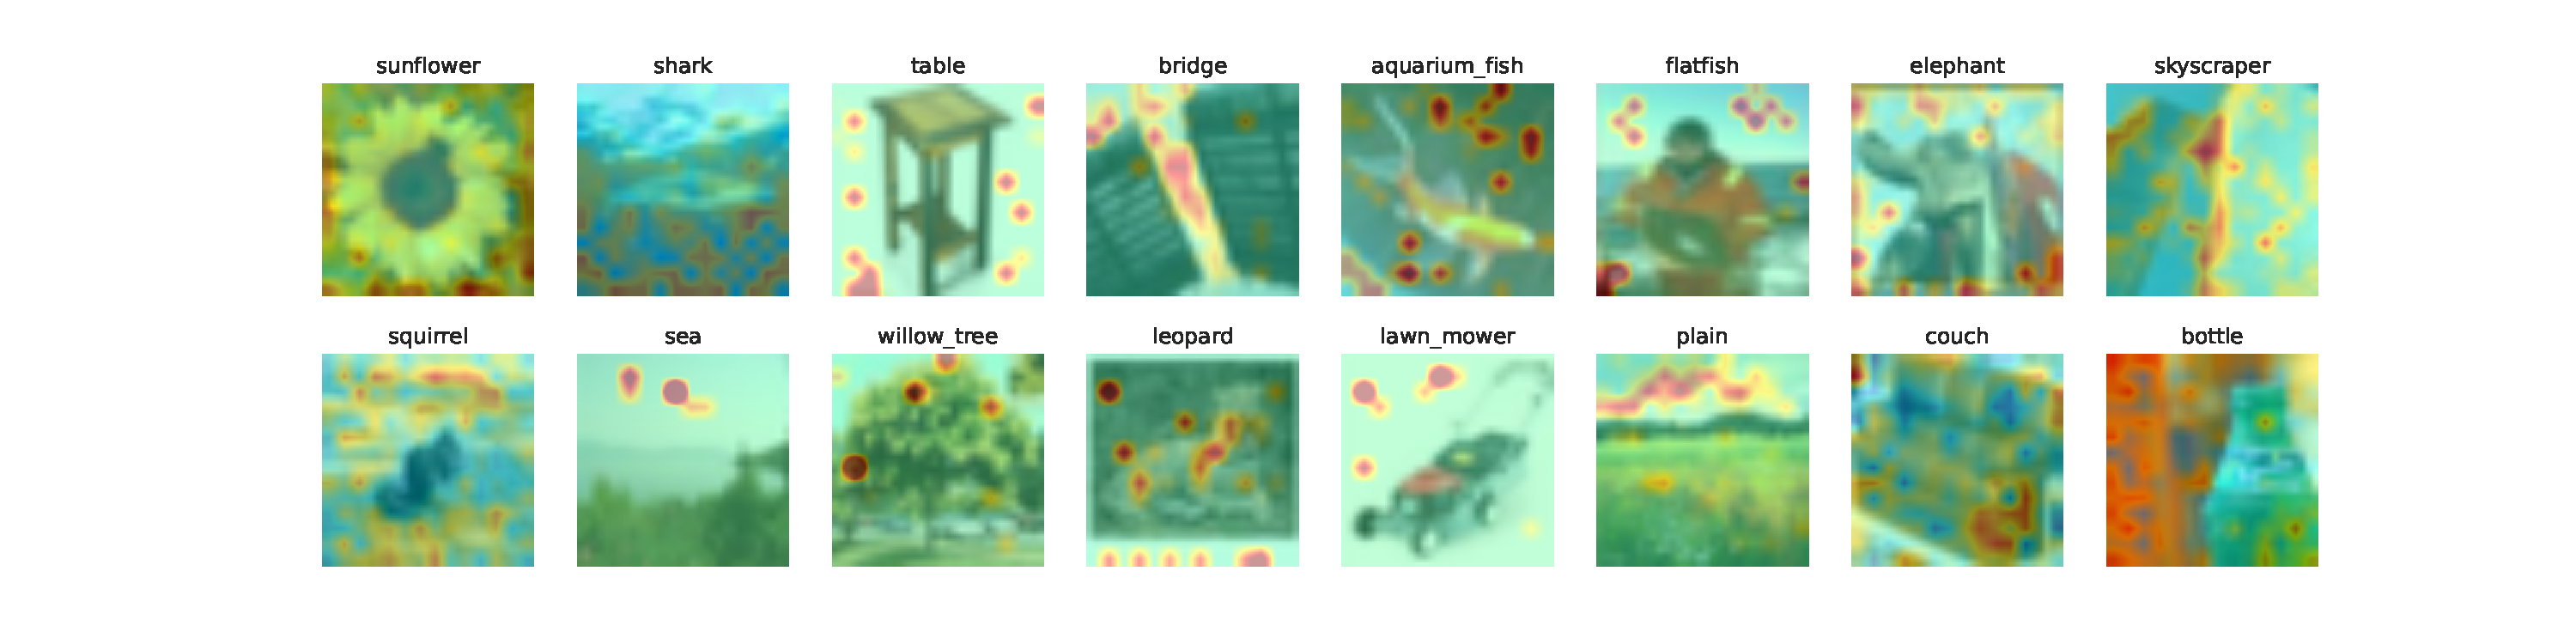
\includegraphics[width=\linewidth]{images/gpp_cifar100_vit_base_patch16_224_noproxy_0.pdf}
            \caption{Without Proxy Attention}
        \end{subfigure}
        \begin{subfigure}[b]{1\textwidth}
            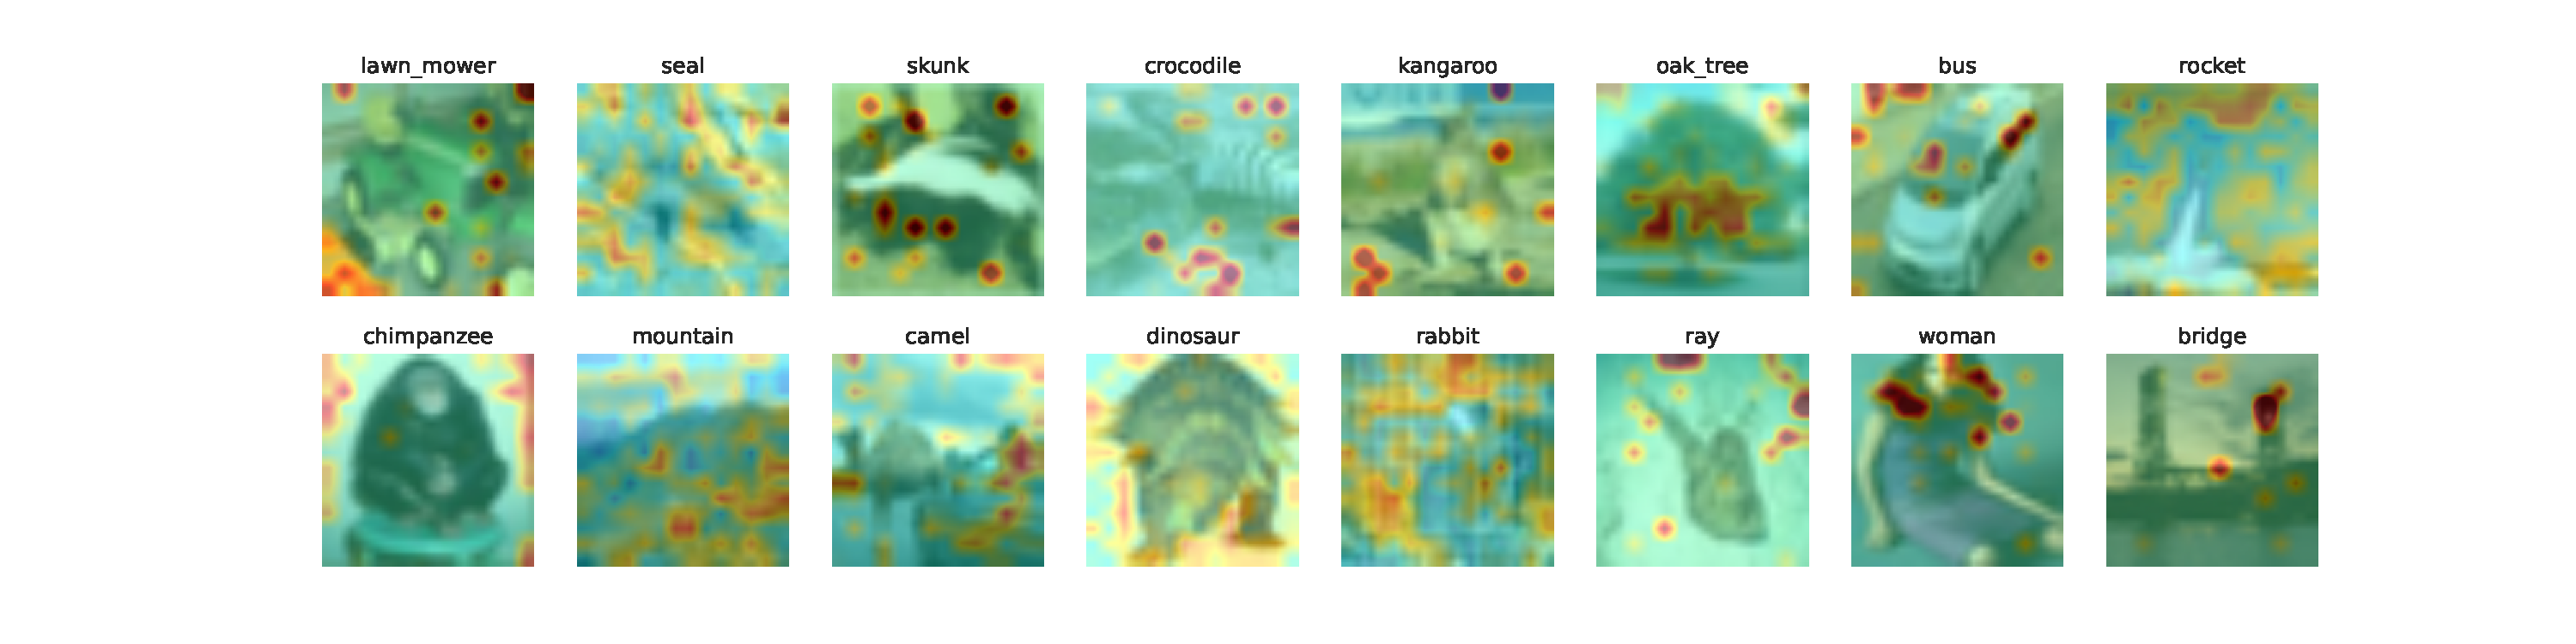
\includegraphics[width=\linewidth]{images/gpp_cifar100_vit_base_patch16_224_proxy_0.pdf}
            \caption{With Proxy Attention}
        \end{subfigure}
        \caption{Comparison of attention maps generated by vit\_base\_patch16\_224 trained with and without Proxy Attention on the cifar100 dataset}
    \end{figure}
    


\subsection{CIFAR 100, ViT , GradCamPlusPlus}
% 
    \begin{figure}[H]
        \centering
        \begin{subfigure}[b]{1\textwidth}
            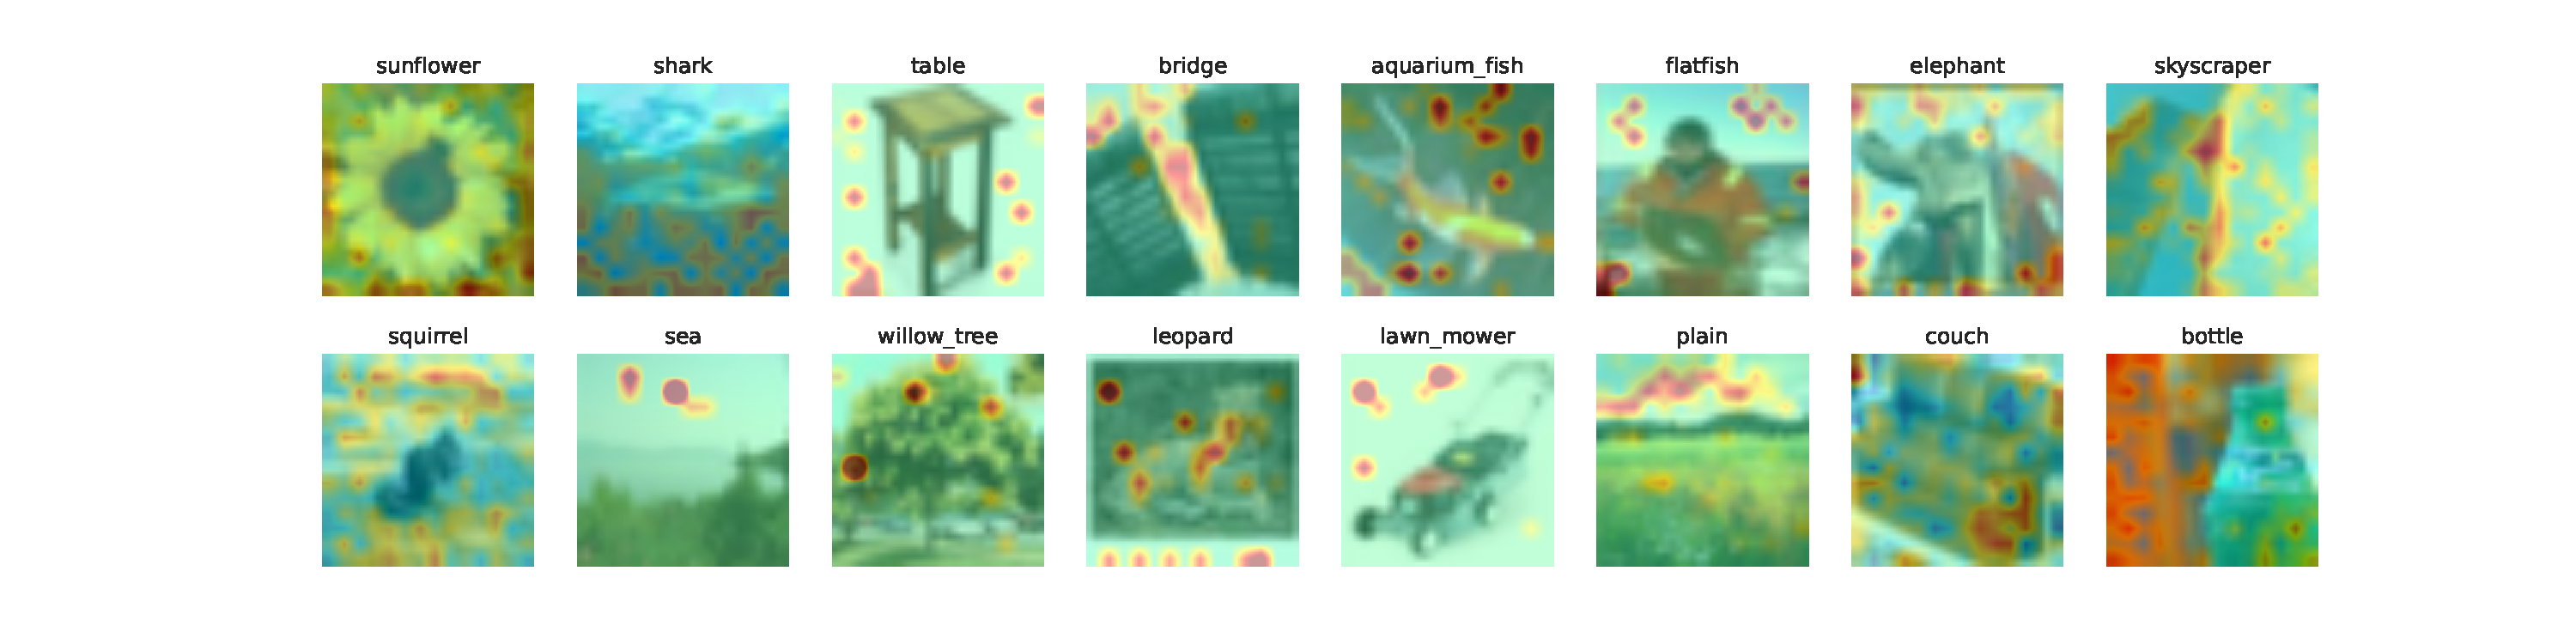
\includegraphics[width=\textwidth]{images/gpp_cifar100_vit_base_patch16_224_noproxy_0.pdf}
            \caption{Without Proxy Attention}
        \end{subfigure}
        \hfill
        \begin{subfigure}[b]{1\textwidth}
            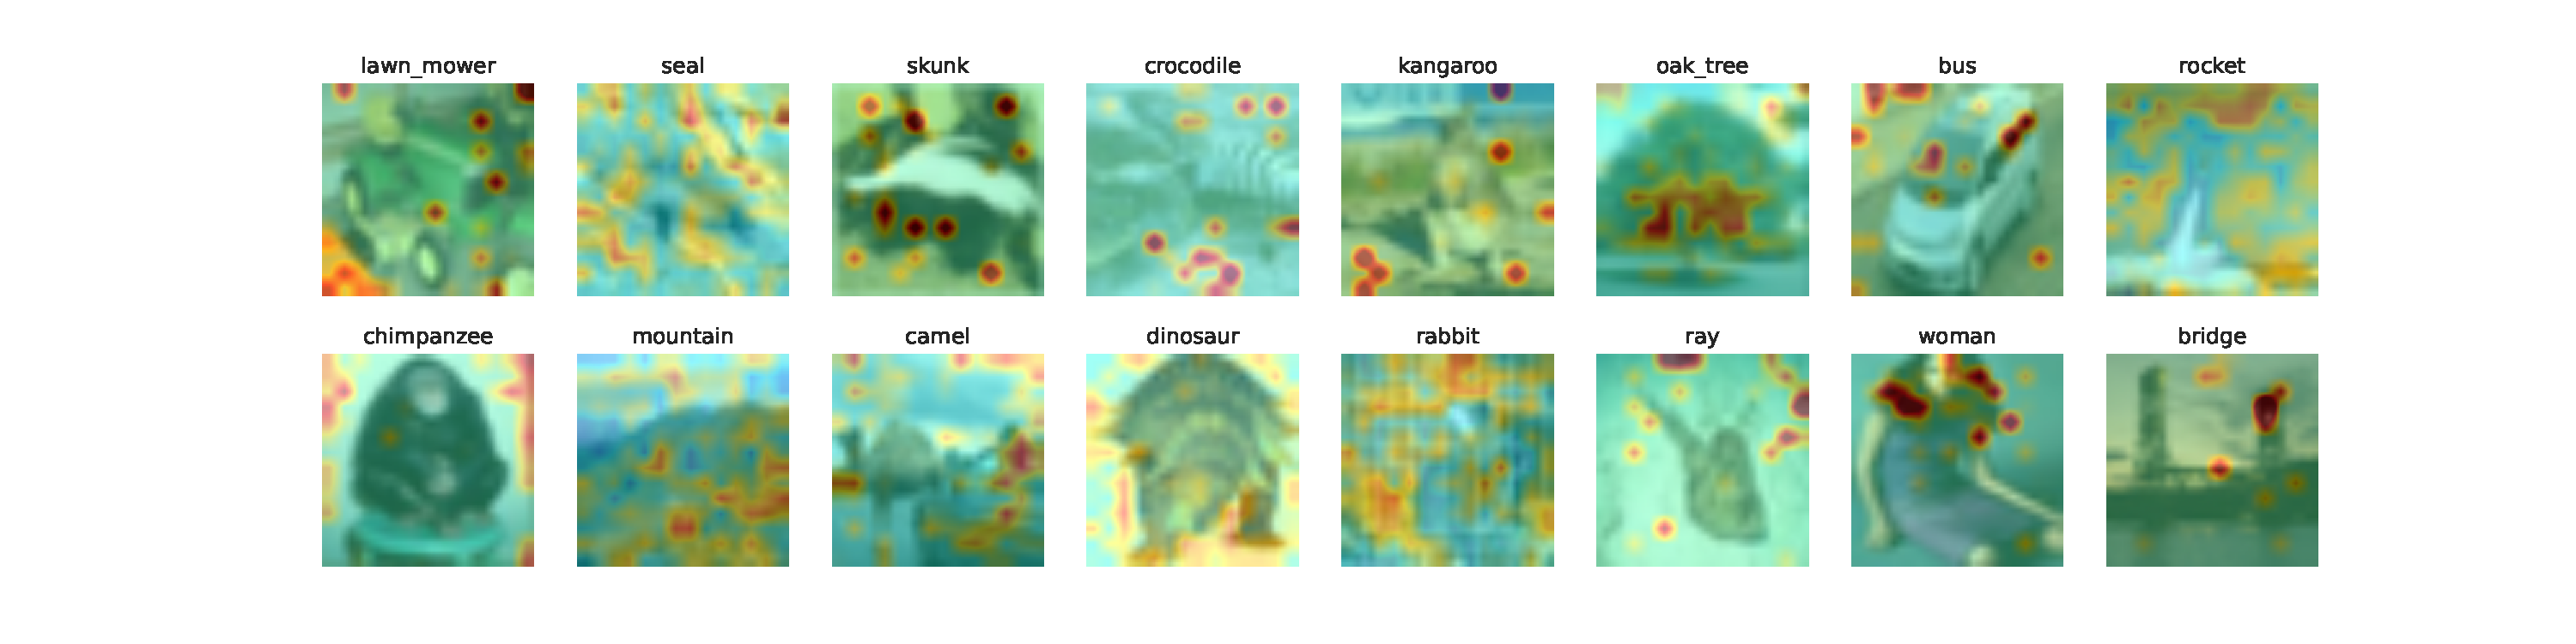
\includegraphics[width=\textwidth]{images/gpp_cifar100_vit_base_patch16_224_proxy_0.pdf}
            \caption{With Proxy Attention}
        \end{subfigure}
        \caption{Comparison of attention maps generated by vit\_base\_patch16\_224 trained with and without Proxy Attention on the cifar100 dataset}
    \end{figure}
    

    \begin{figure}[H]
        \centering
        \begin{subfigure}[b]{1\textwidth}
            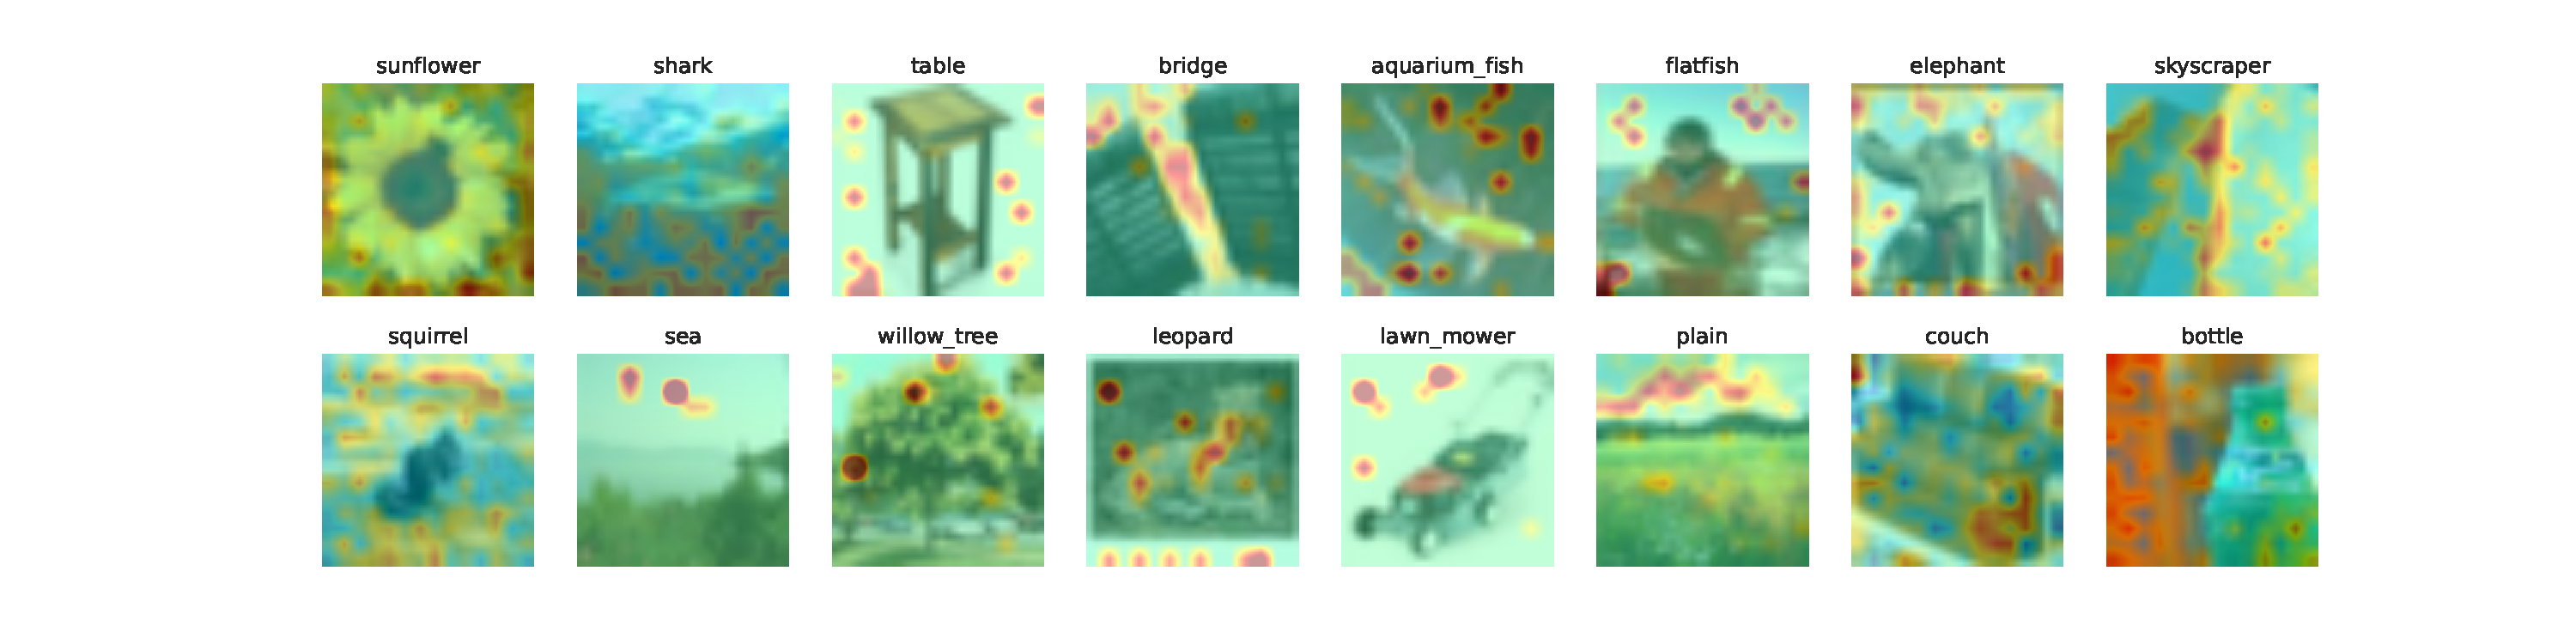
\includegraphics[width=\textwidth]{images/gpp_cifar100_vit_base_patch16_224_noproxy_0.pdf}
            \caption{Without Proxy Attention}
        \end{subfigure}
        \hfill
        \begin{subfigure}[b]{1\textwidth}
            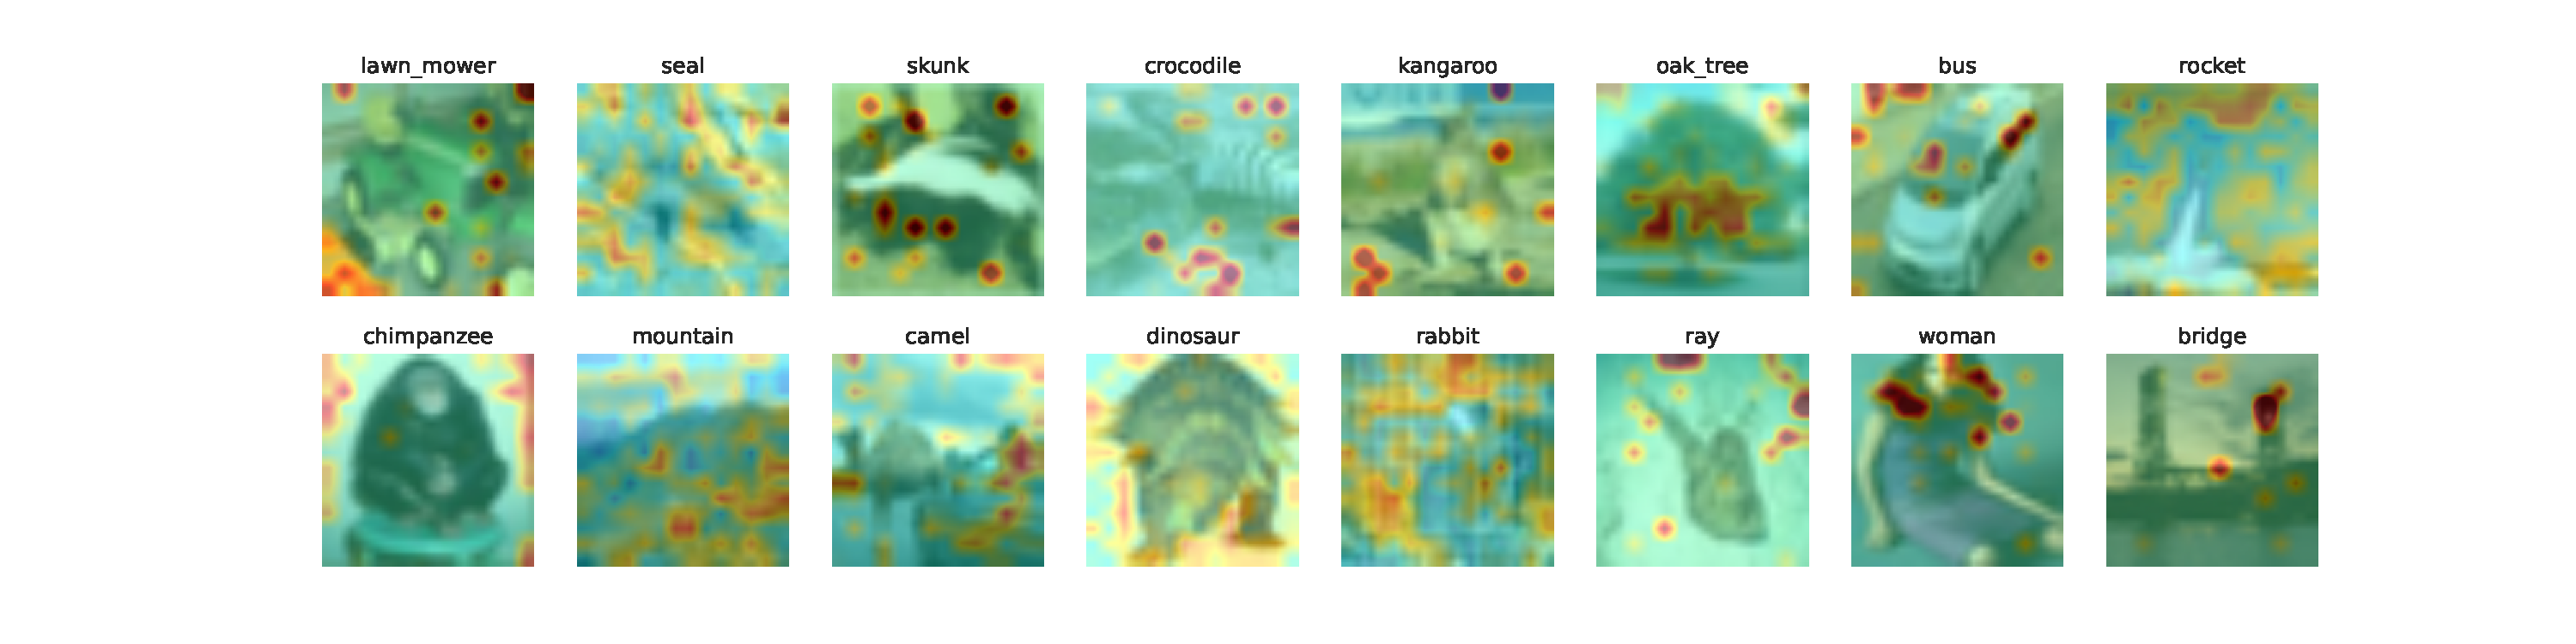
\includegraphics[width=\textwidth]{images/gpp_cifar100_vit_base_patch16_224_proxy_0.pdf}
            \caption{With Proxy Attention}
        \end{subfigure}
        \caption{Comparison of attention maps generated by vit\_base\_patch16\_224 trained with and without Proxy Attention on the cifar100 dataset}
    \end{figure}
    

    \begin{figure}[H]
        \centering
        \begin{subfigure}[b]{1\textwidth}
            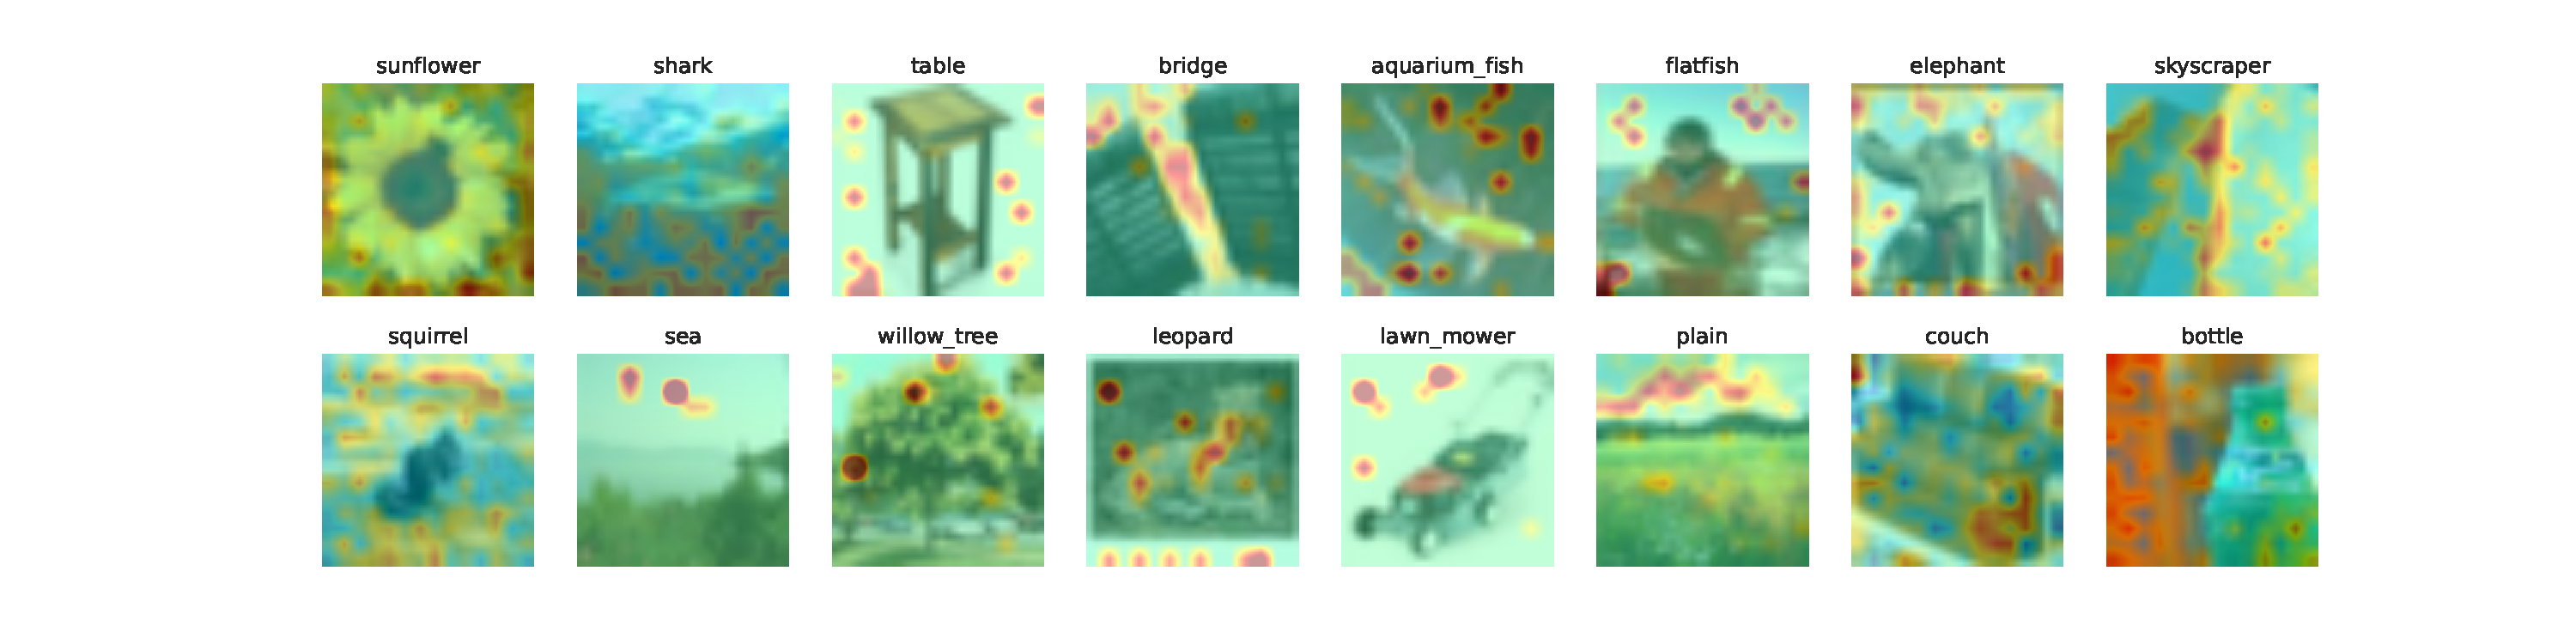
\includegraphics[width=\textwidth]{images/gpp_cifar100_vit_base_patch16_224_noproxy_0.pdf}
            \caption{Without Proxy Attention}
        \end{subfigure}
        \hfill
        \begin{subfigure}[b]{1\textwidth}
            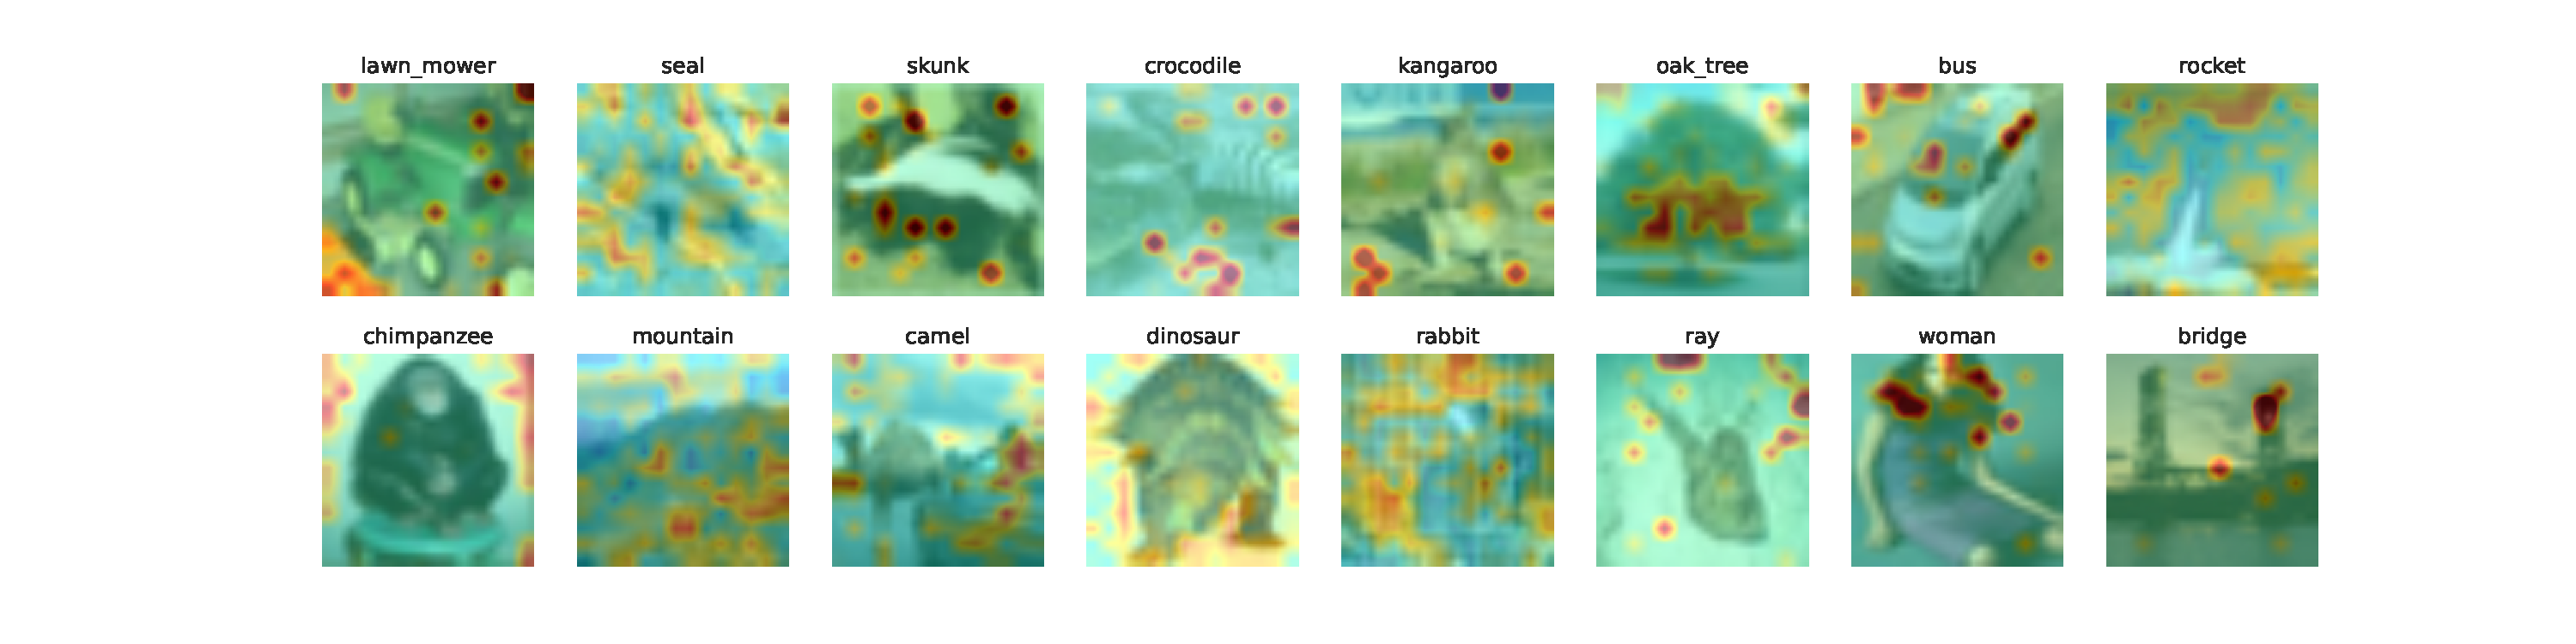
\includegraphics[width=\textwidth]{images/gpp_cifar100_vit_base_patch16_224_proxy_0.pdf}
            \caption{With Proxy Attention}
        \end{subfigure}
        \caption{Comparison of attention maps generated by vit\_base\_patch16\_224 trained with and without Proxy Attention on the cifar100 dataset}
    \end{figure}
    

    \begin{figure}[H]
        \centering
        \begin{subfigure}[b]{1\textwidth}
            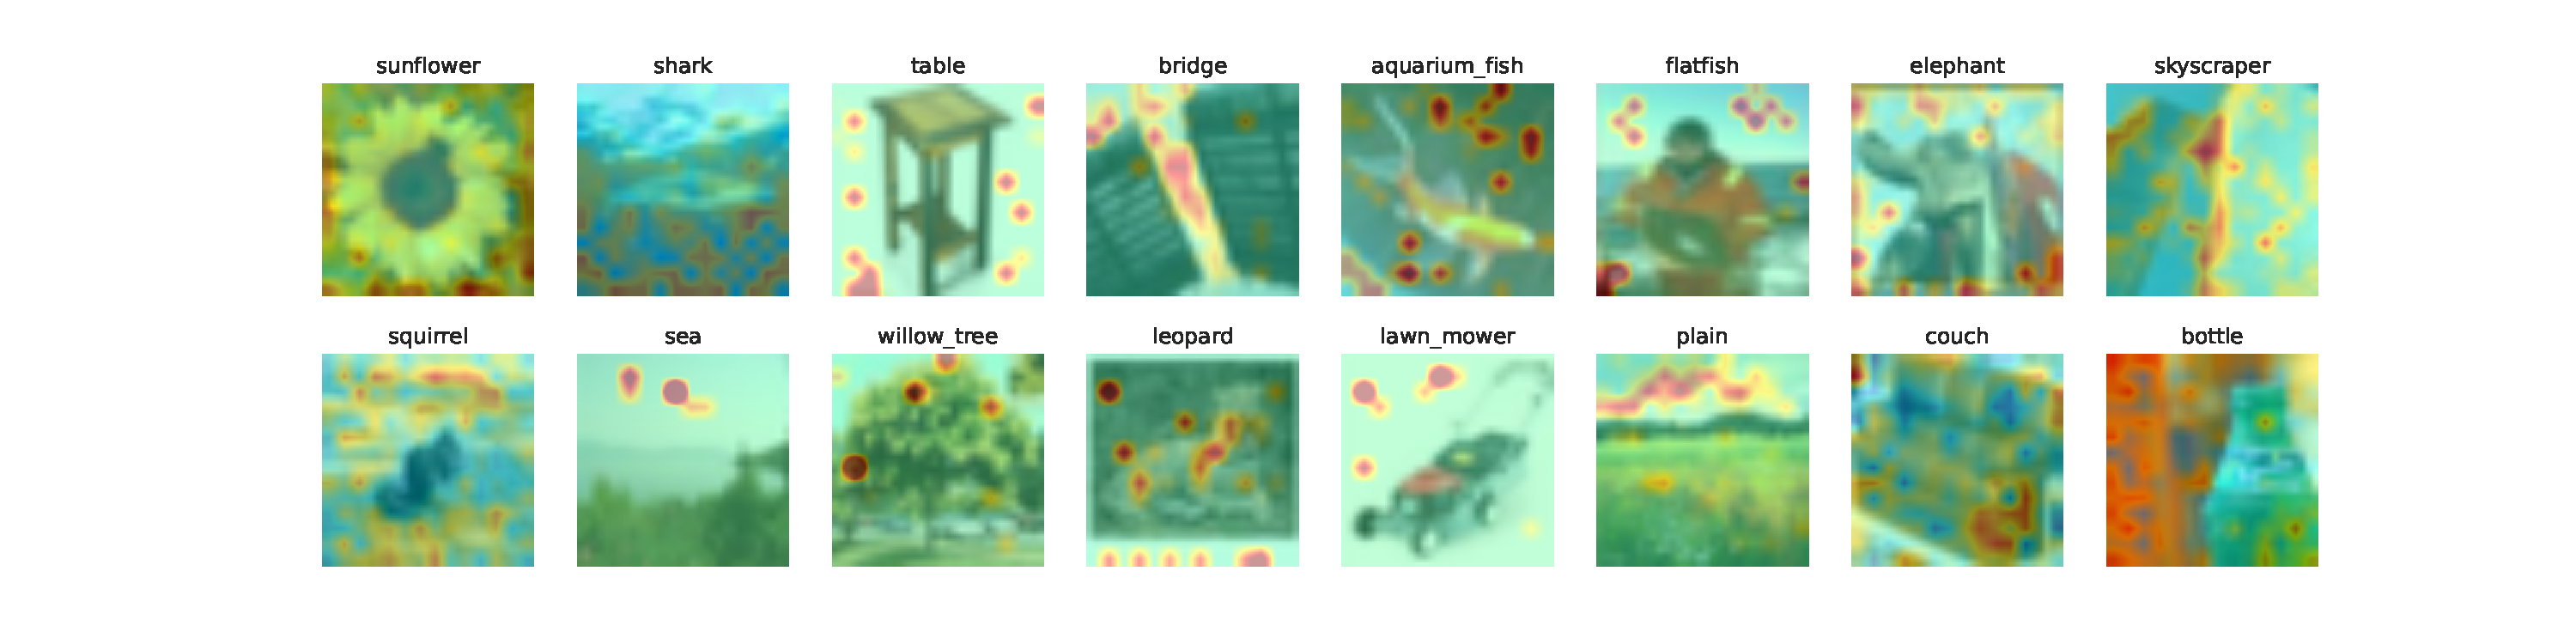
\includegraphics[width=\textwidth]{images/gpp_cifar100_vit_base_patch16_224_noproxy_0.pdf}
            \caption{Without Proxy Attention}
        \end{subfigure}
        \hfill
        \begin{subfigure}[b]{1\textwidth}
            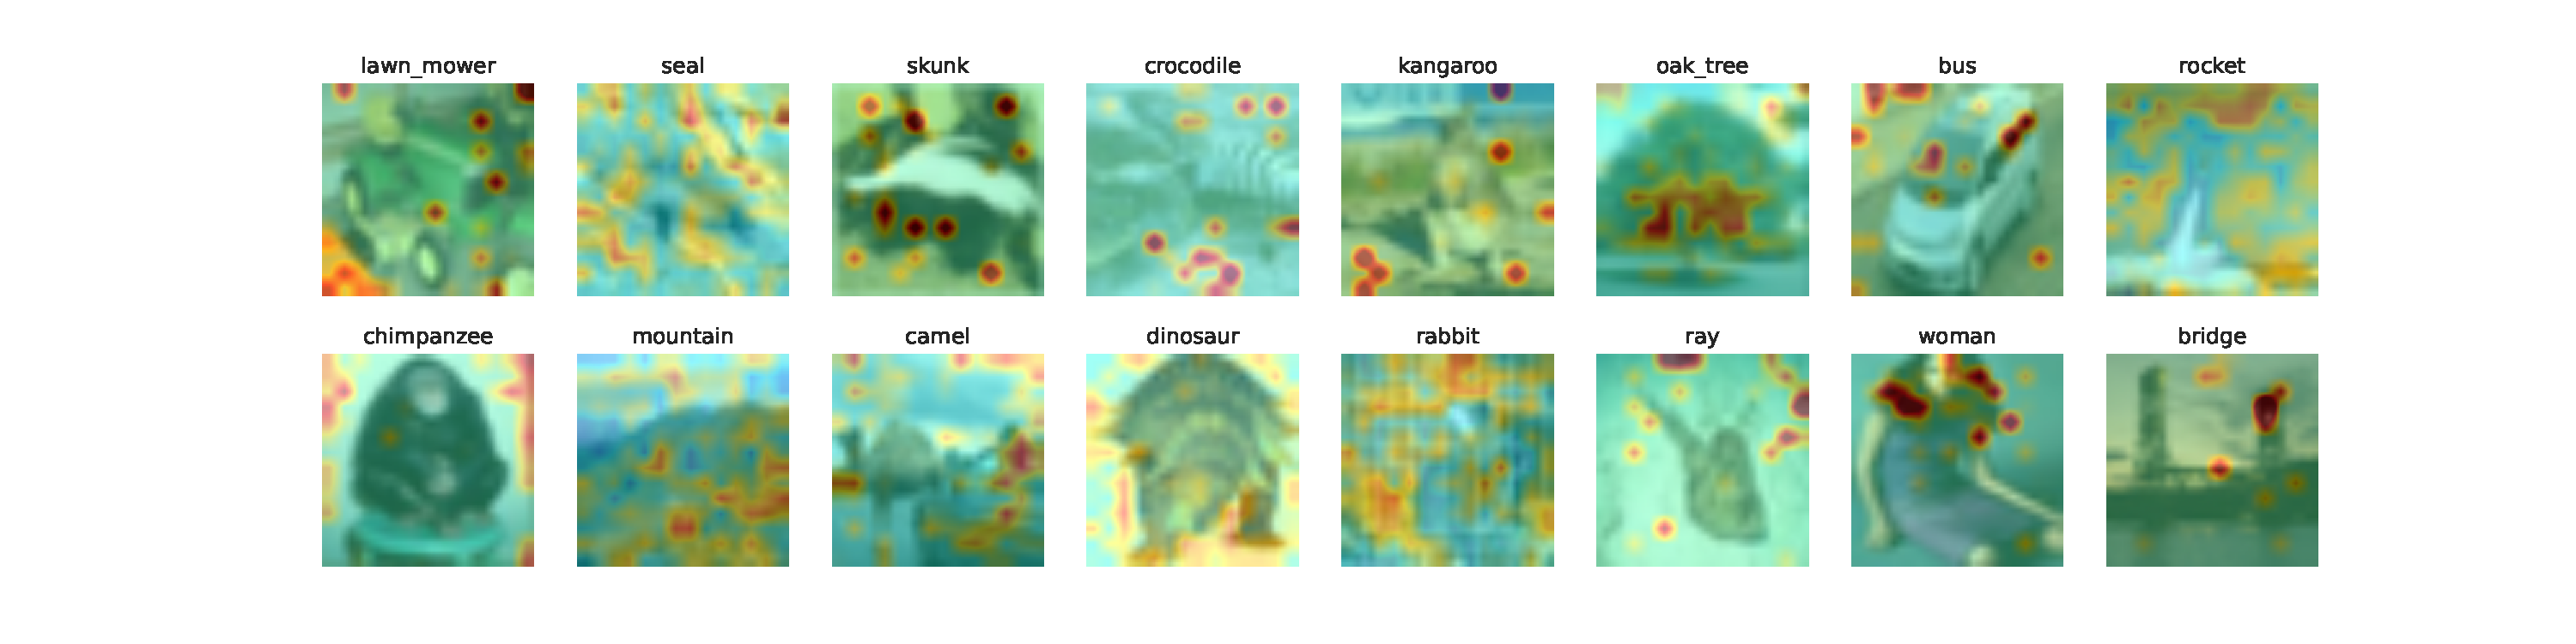
\includegraphics[width=\textwidth]{images/gpp_cifar100_vit_base_patch16_224_proxy_0.pdf}
            \caption{With Proxy Attention}
        \end{subfigure}
        \caption{Comparison of attention maps generated by vit\_base\_patch16\_224 trained with and without Proxy Attention on the cifar100 dataset}
    \end{figure}
    

\begin{figure}[H]
        \begin{subfigure}[b]{1\textwidth}
            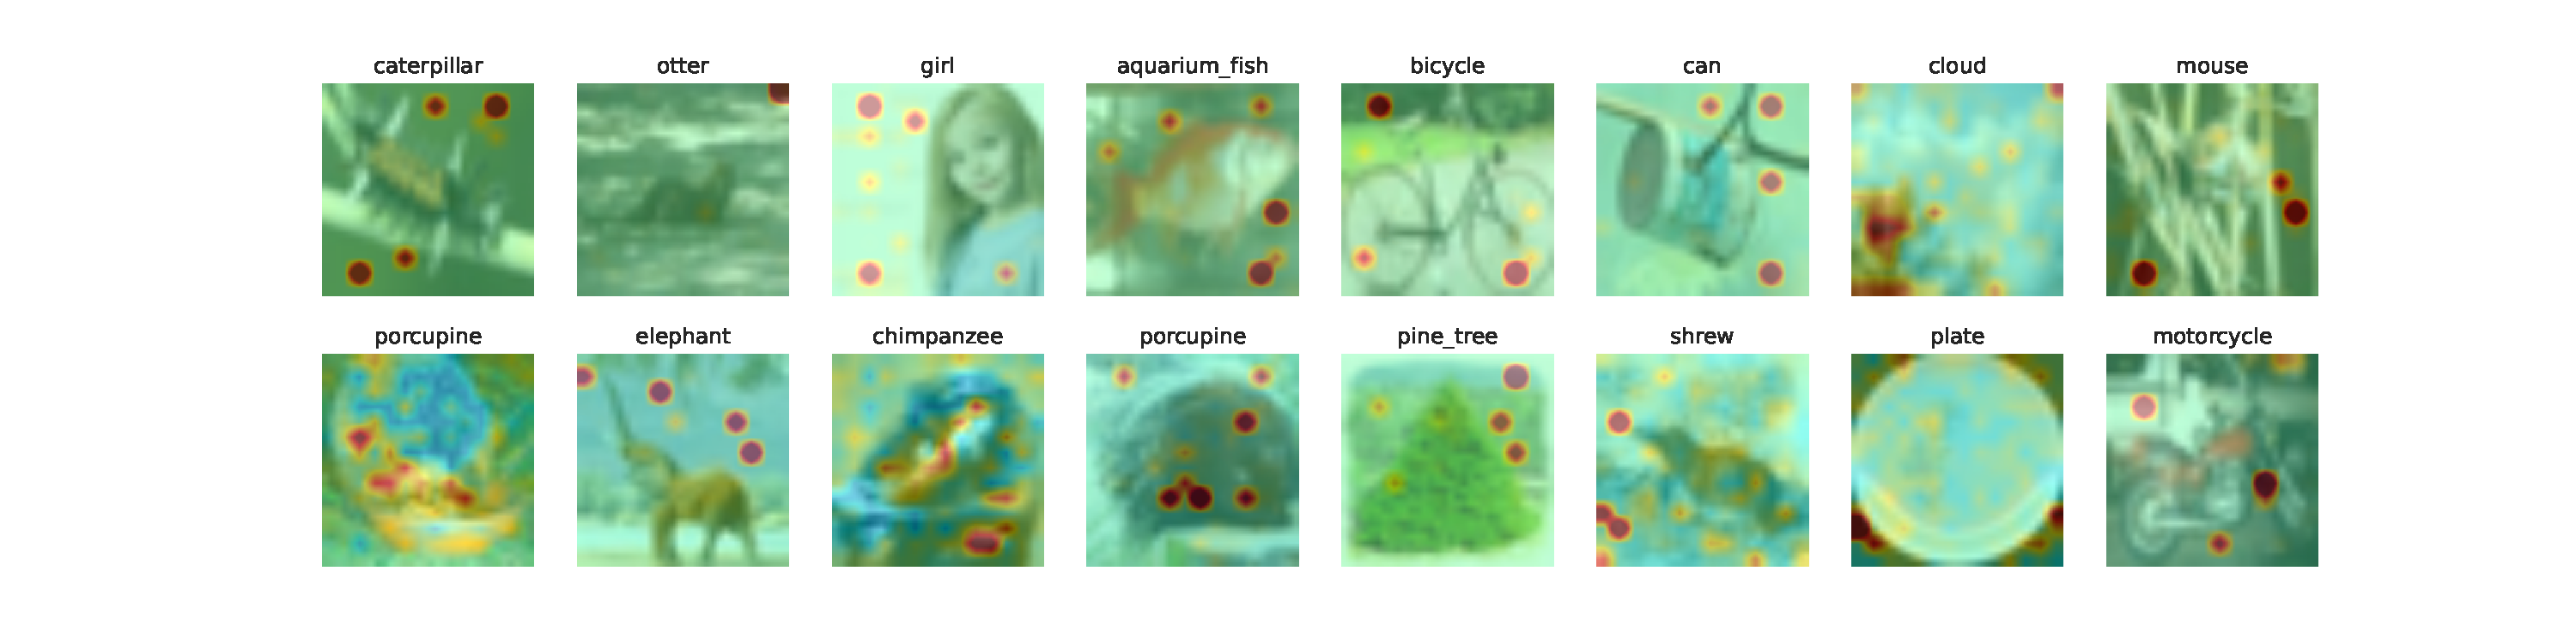
\includegraphics[width=\linewidth]{images/cifar100_vit_base_patch16_224_noproxy_0.pdf}
            \caption{Without Proxy Attention}
        \end{subfigure}
        \begin{subfigure}[b]{1\textwidth}
            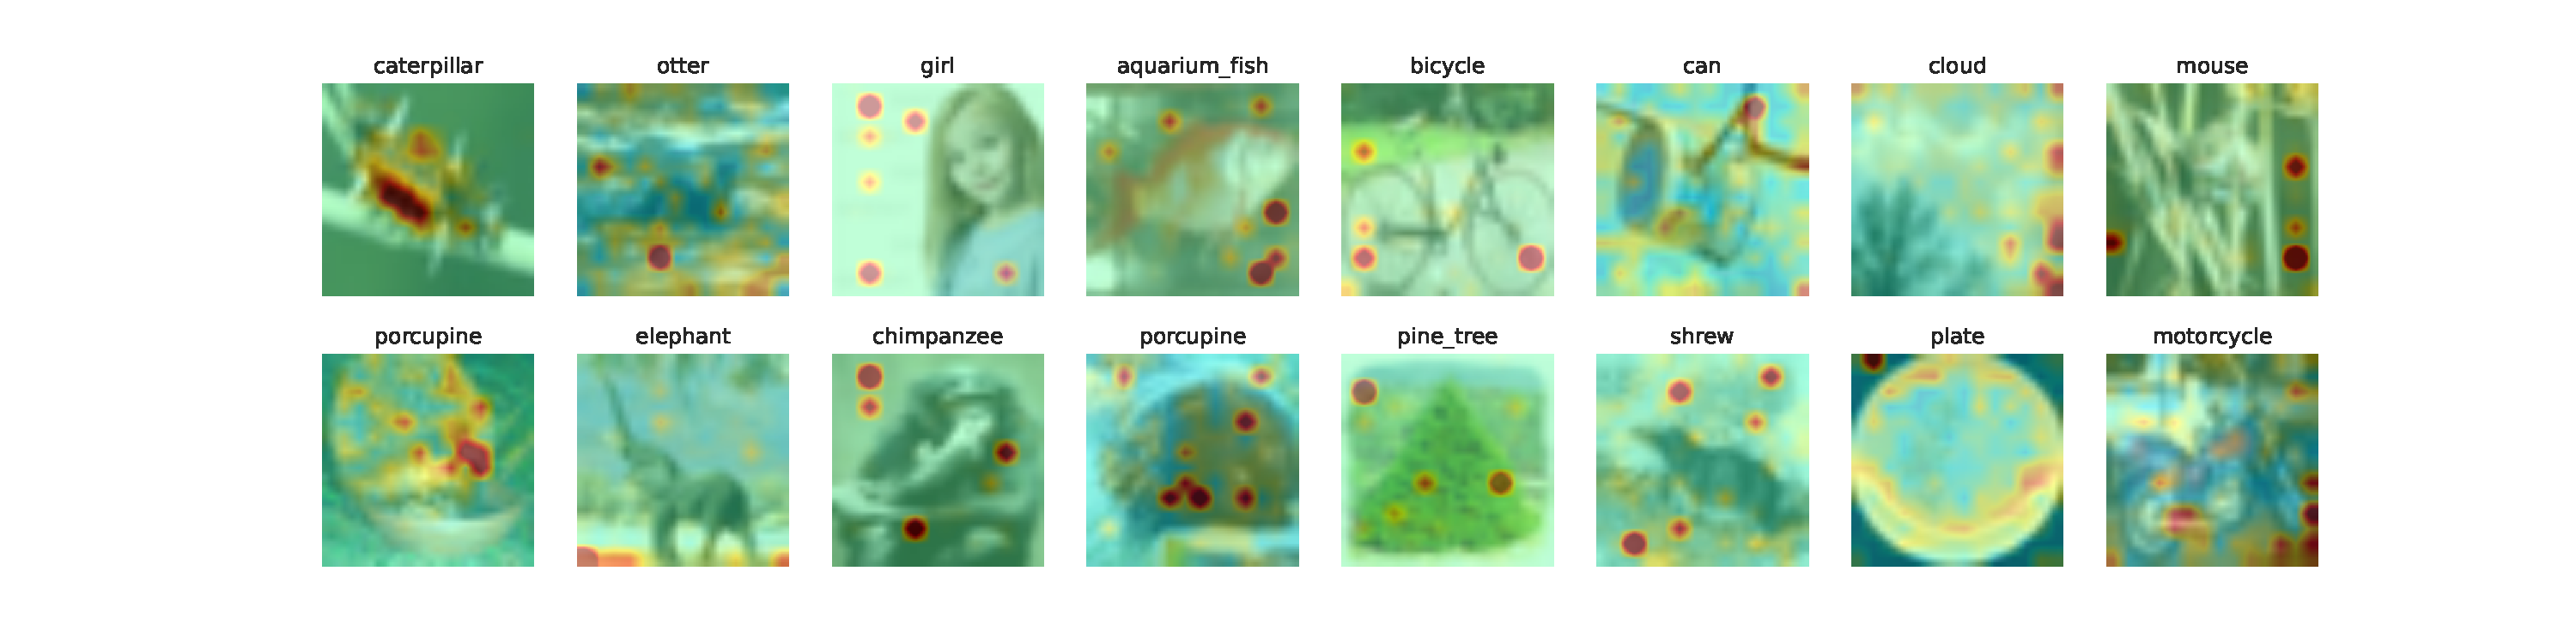
\includegraphics[width=\linewidth]{images/cifar100_vit_base_patch16_224_proxy_0.pdf}
            \caption{With Proxy Attention}
        \end{subfigure}
        \caption{Comparison of attention maps generated by vit\_base\_patch16\_224 trained with and without Proxy Attention on the cifar100 dataset}
    \end{figure}
    


\subsection{Tsinghua Dogs, ResNet50 , GradCamPlusPlus}
% 
    \begin{figure}[H]
        \centering
        \begin{subfigure}[b]{1\textwidth}
            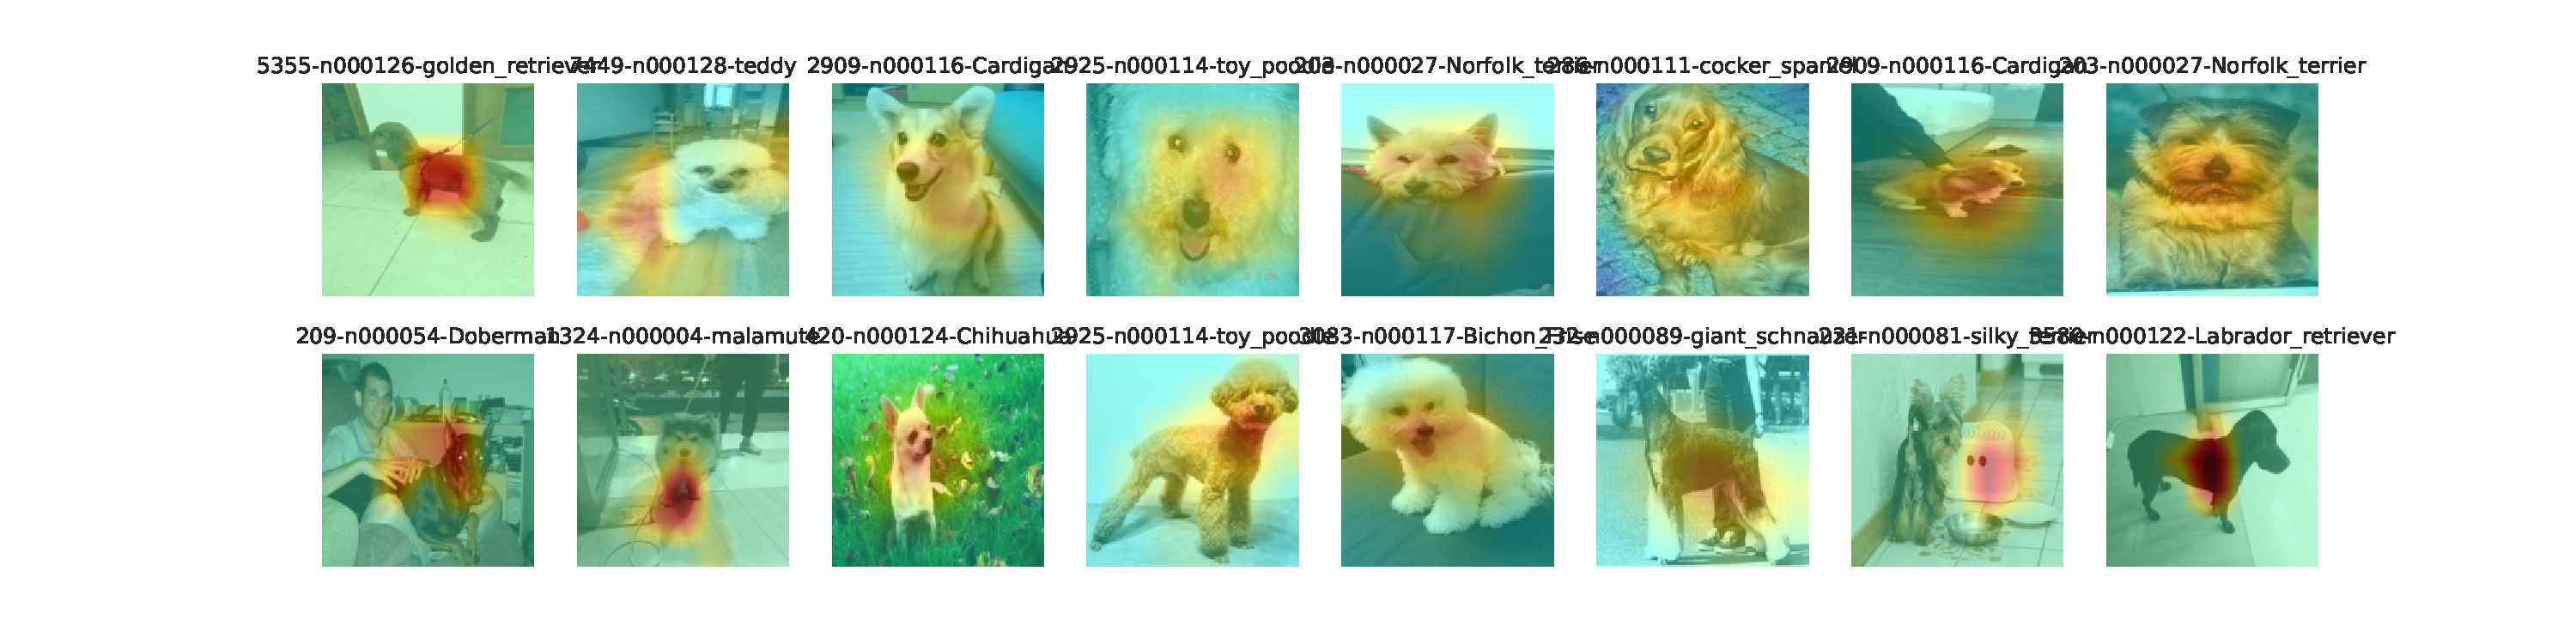
\includegraphics[width=\textwidth]{images/gpp_tsing_resnet50_noproxy_0.pdf}
            \caption{Without Proxy Attention}
        \end{subfigure}
        \hfill
        \begin{subfigure}[b]{1\textwidth}
            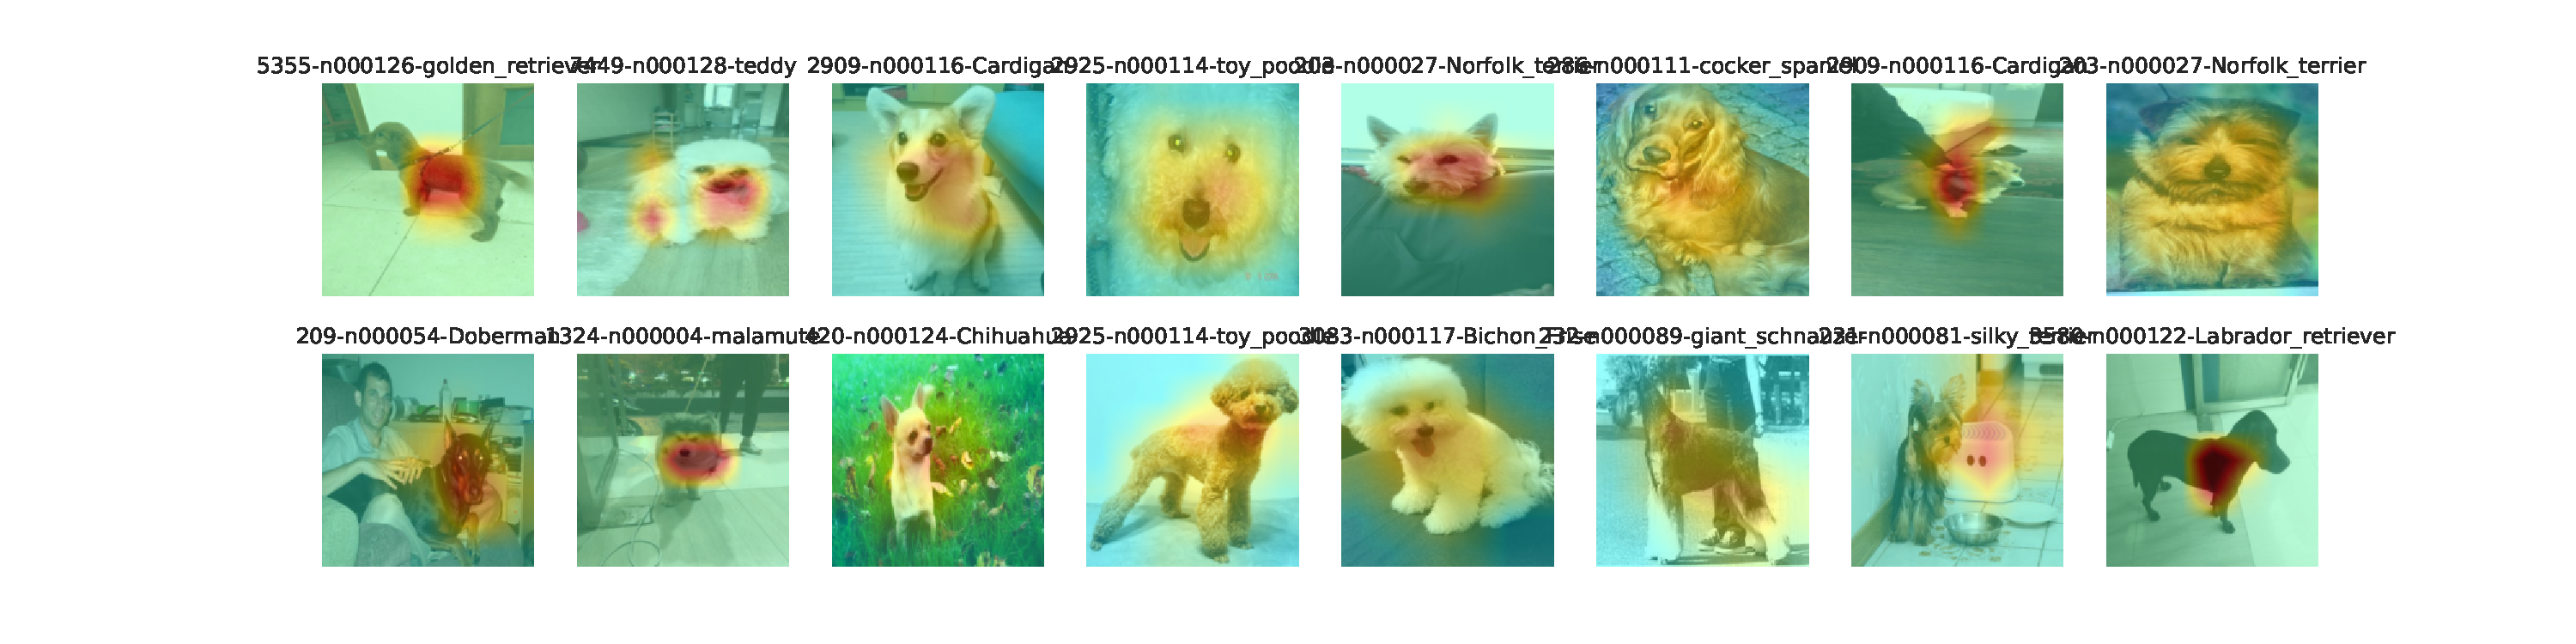
\includegraphics[width=\textwidth]{images/gpp_tsing_resnet50_proxy_0.pdf}
            \caption{With Proxy Attention}
        \end{subfigure}
        \caption{Comparison of attention maps generated by resnet50 trained with and without Proxy Attention on the tsing dataset}
    \end{figure}
    

    \begin{figure}[H]
        \centering
        \begin{subfigure}[b]{1\textwidth}
            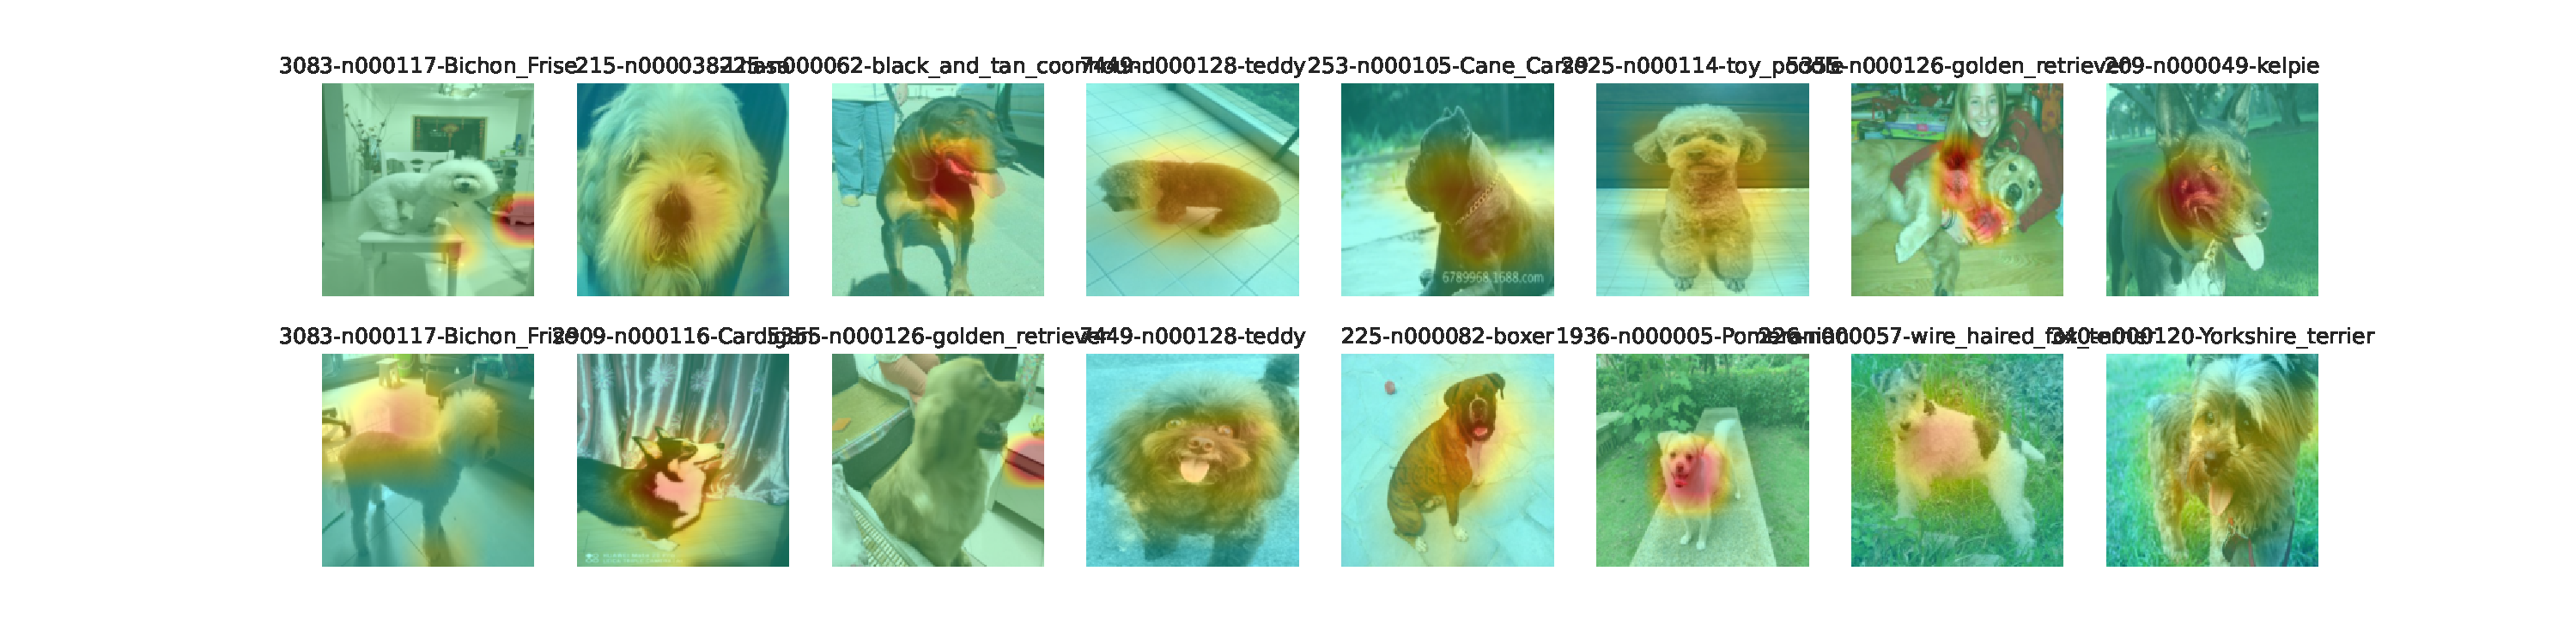
\includegraphics[width=\textwidth]{images/gpp_tsing_resnet50_noproxy_1.pdf}
            \caption{Without Proxy Attention}
        \end{subfigure}
        \hfill
        \begin{subfigure}[b]{1\textwidth}
            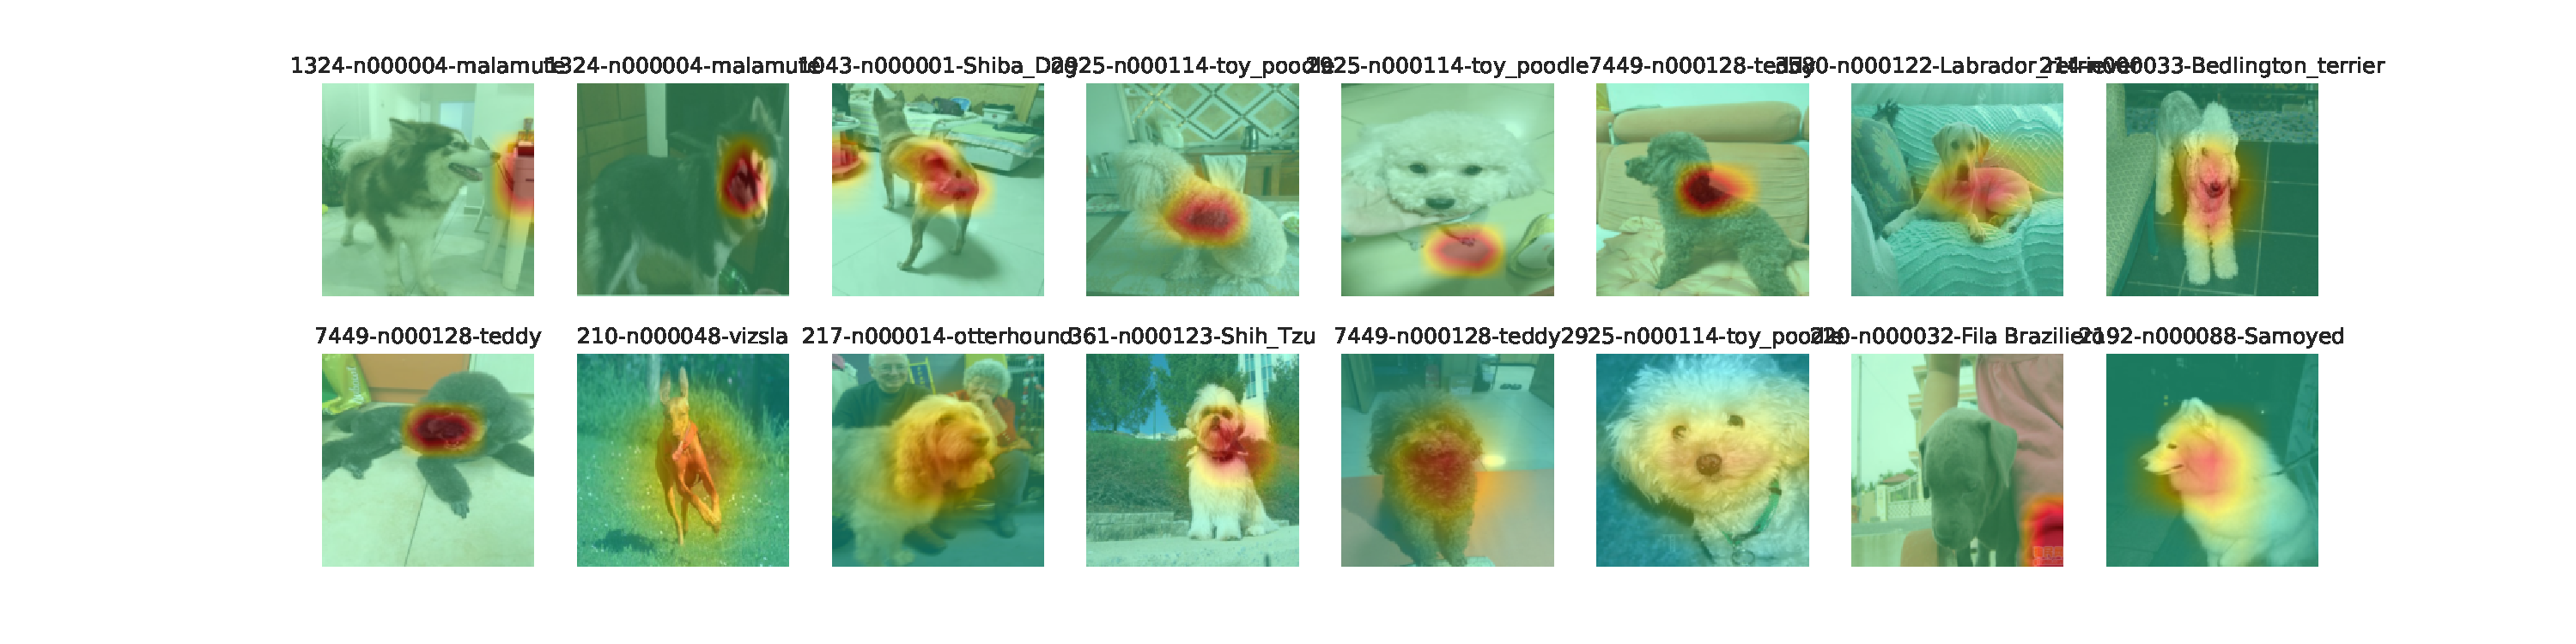
\includegraphics[width=\textwidth]{images/gpp_tsing_resnet50_proxy_1.pdf}
            \caption{With Proxy Attention}
        \end{subfigure}
        \caption{Comparison of attention maps generated by resnet50 trained with and without Proxy Attention on the tsing dataset}
    \end{figure}
    

    \begin{figure}[H]
        \centering
        \begin{subfigure}[b]{1\textwidth}
            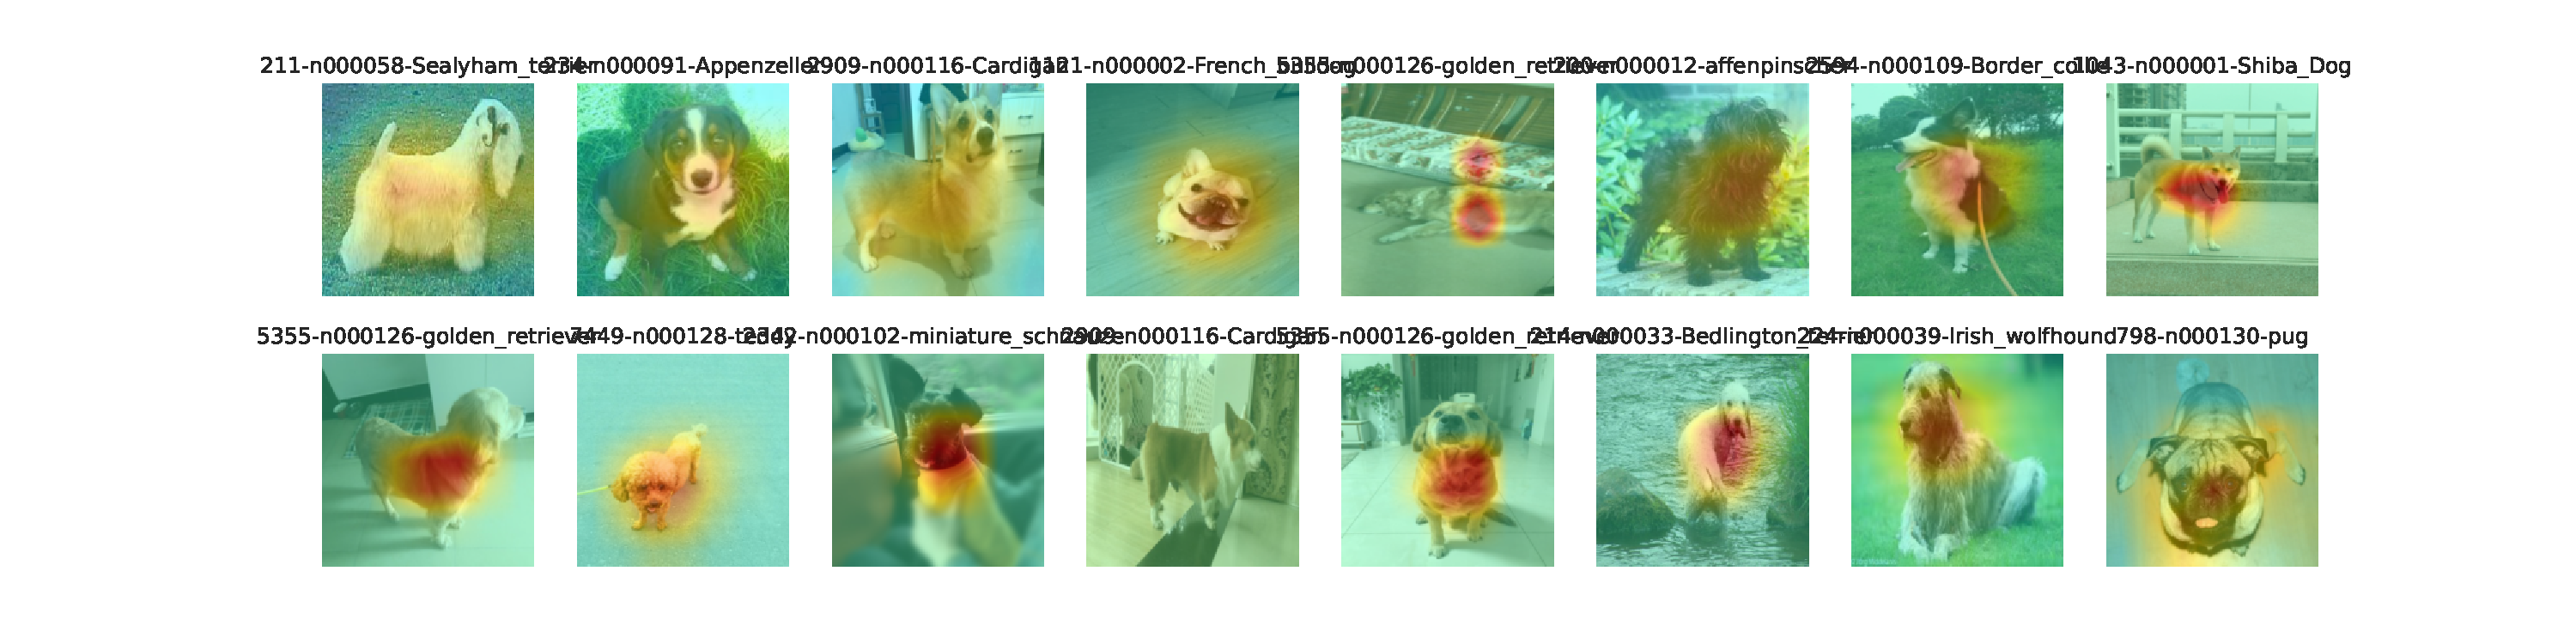
\includegraphics[width=\textwidth]{images/gpp_tsing_resnet50_noproxy_2.pdf}
            \caption{Without Proxy Attention}
        \end{subfigure}
        \hfill
        \begin{subfigure}[b]{1\textwidth}
            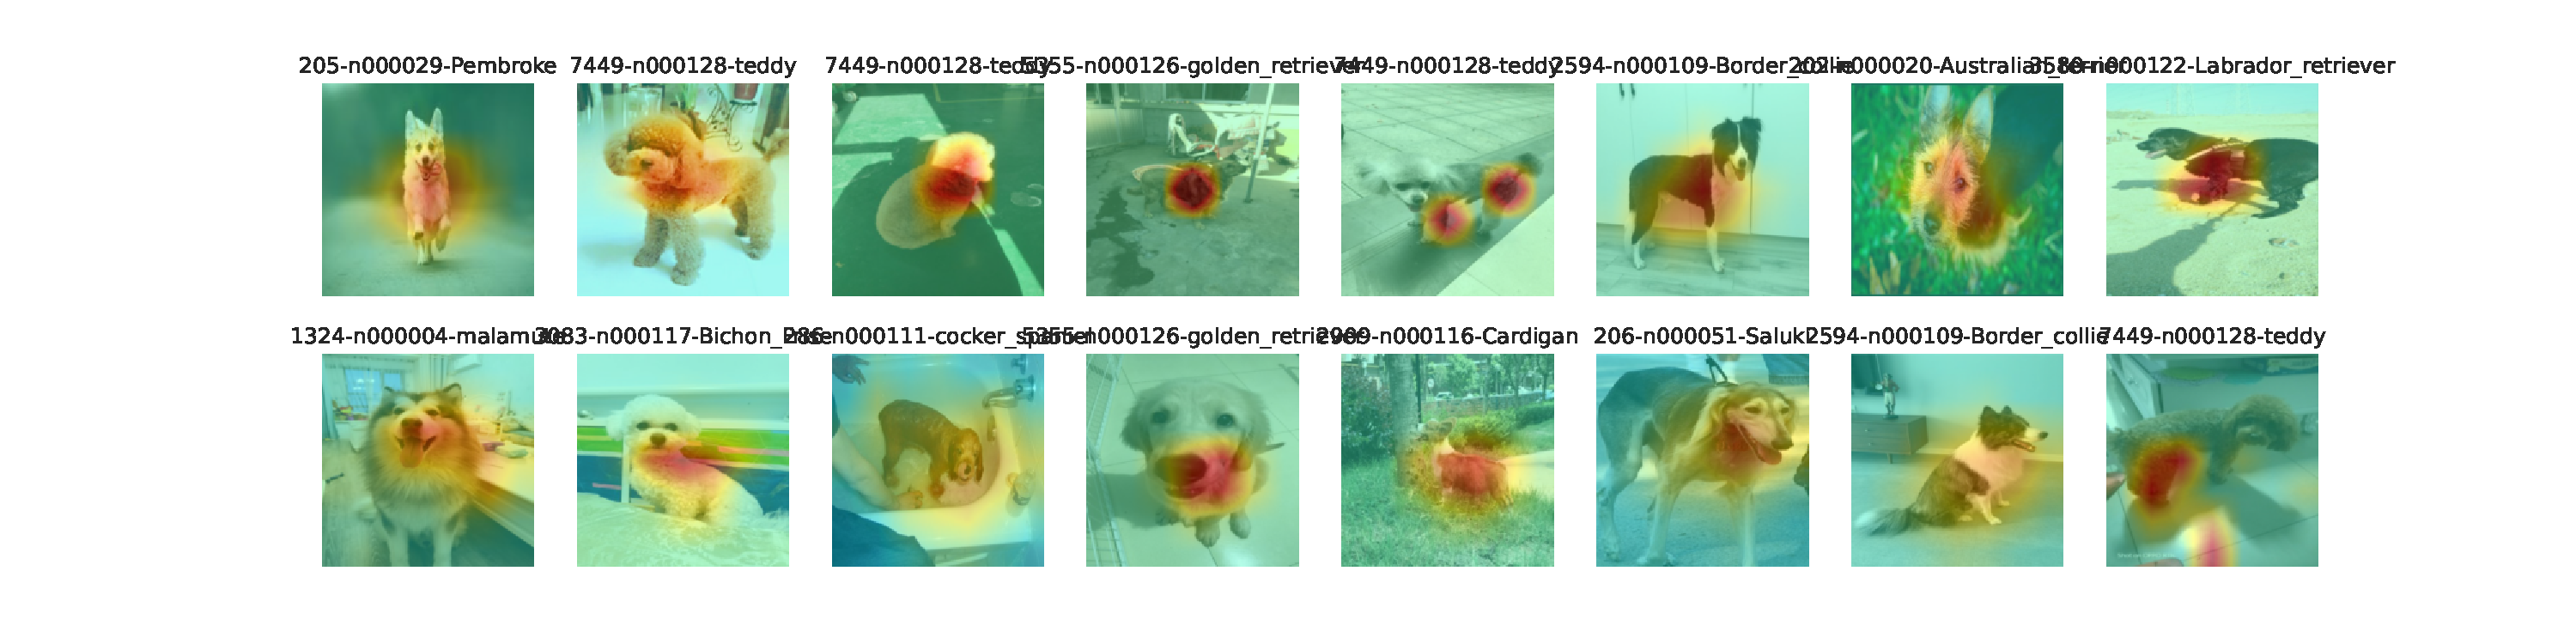
\includegraphics[width=\textwidth]{images/gpp_tsing_resnet50_proxy_2.pdf}
            \caption{With Proxy Attention}
        \end{subfigure}
        \caption{Comparison of attention maps generated by resnet50 trained with and without Proxy Attention on the tsing dataset}
    \end{figure}
    

    \begin{figure}[H]
        \centering
        \begin{subfigure}[b]{1\textwidth}
            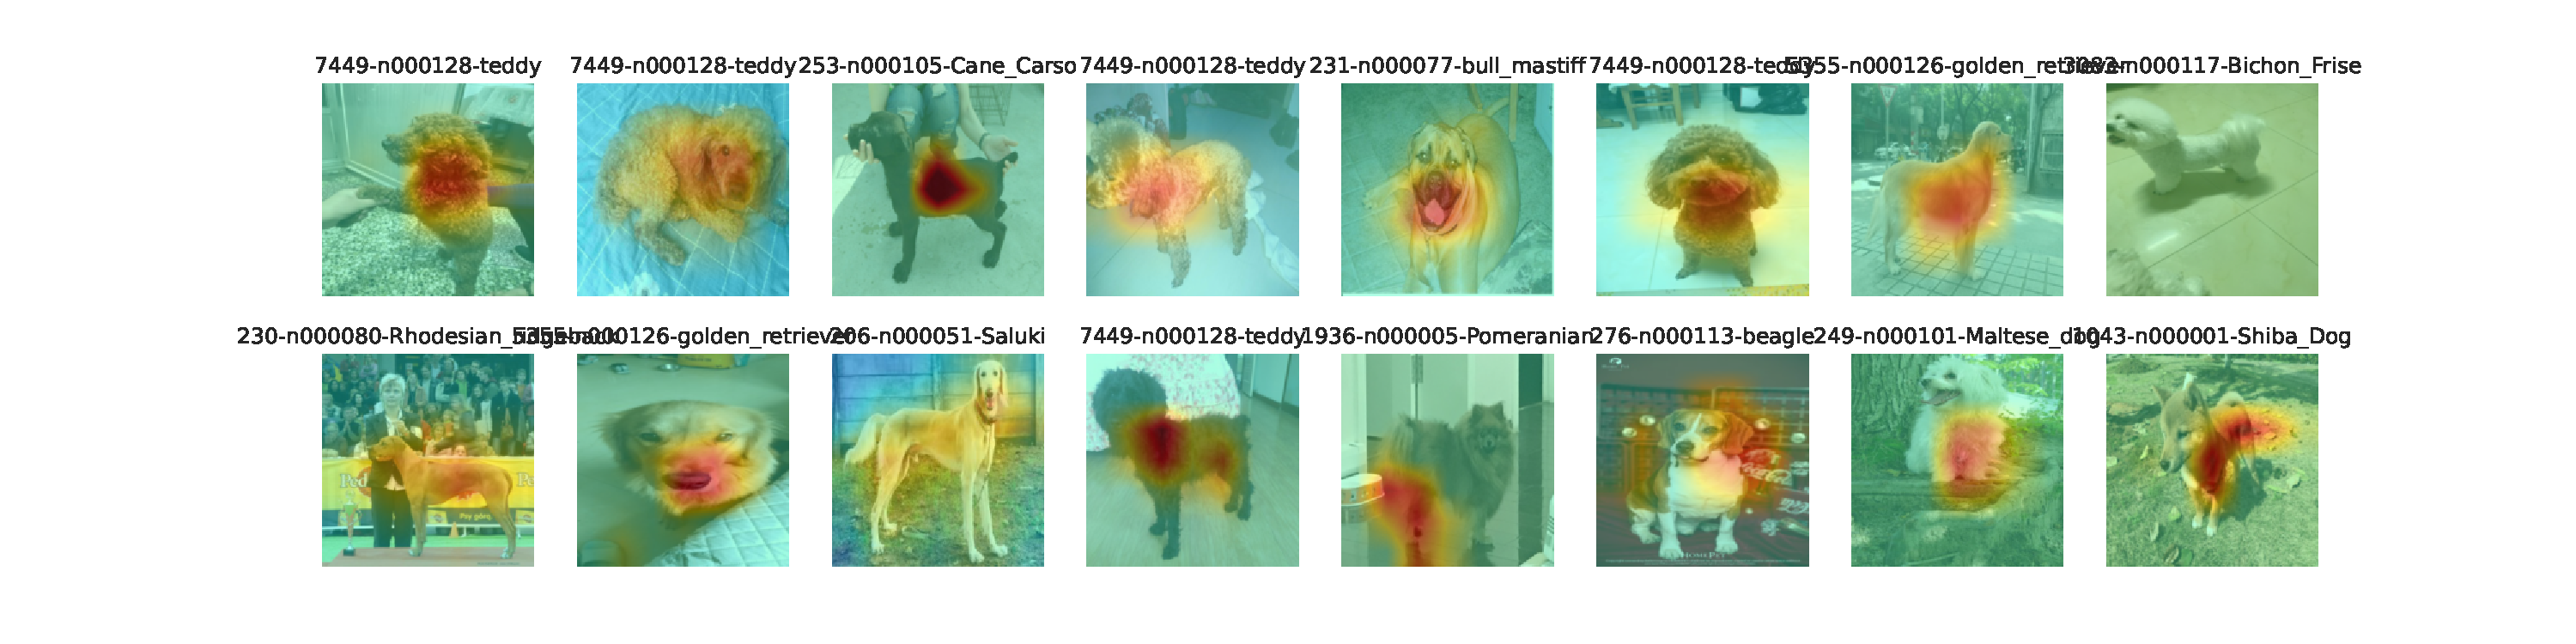
\includegraphics[width=\textwidth]{images/gpp_tsing_resnet50_noproxy_3.pdf}
            \caption{Without Proxy Attention}
        \end{subfigure}
        \hfill
        \begin{subfigure}[b]{1\textwidth}
            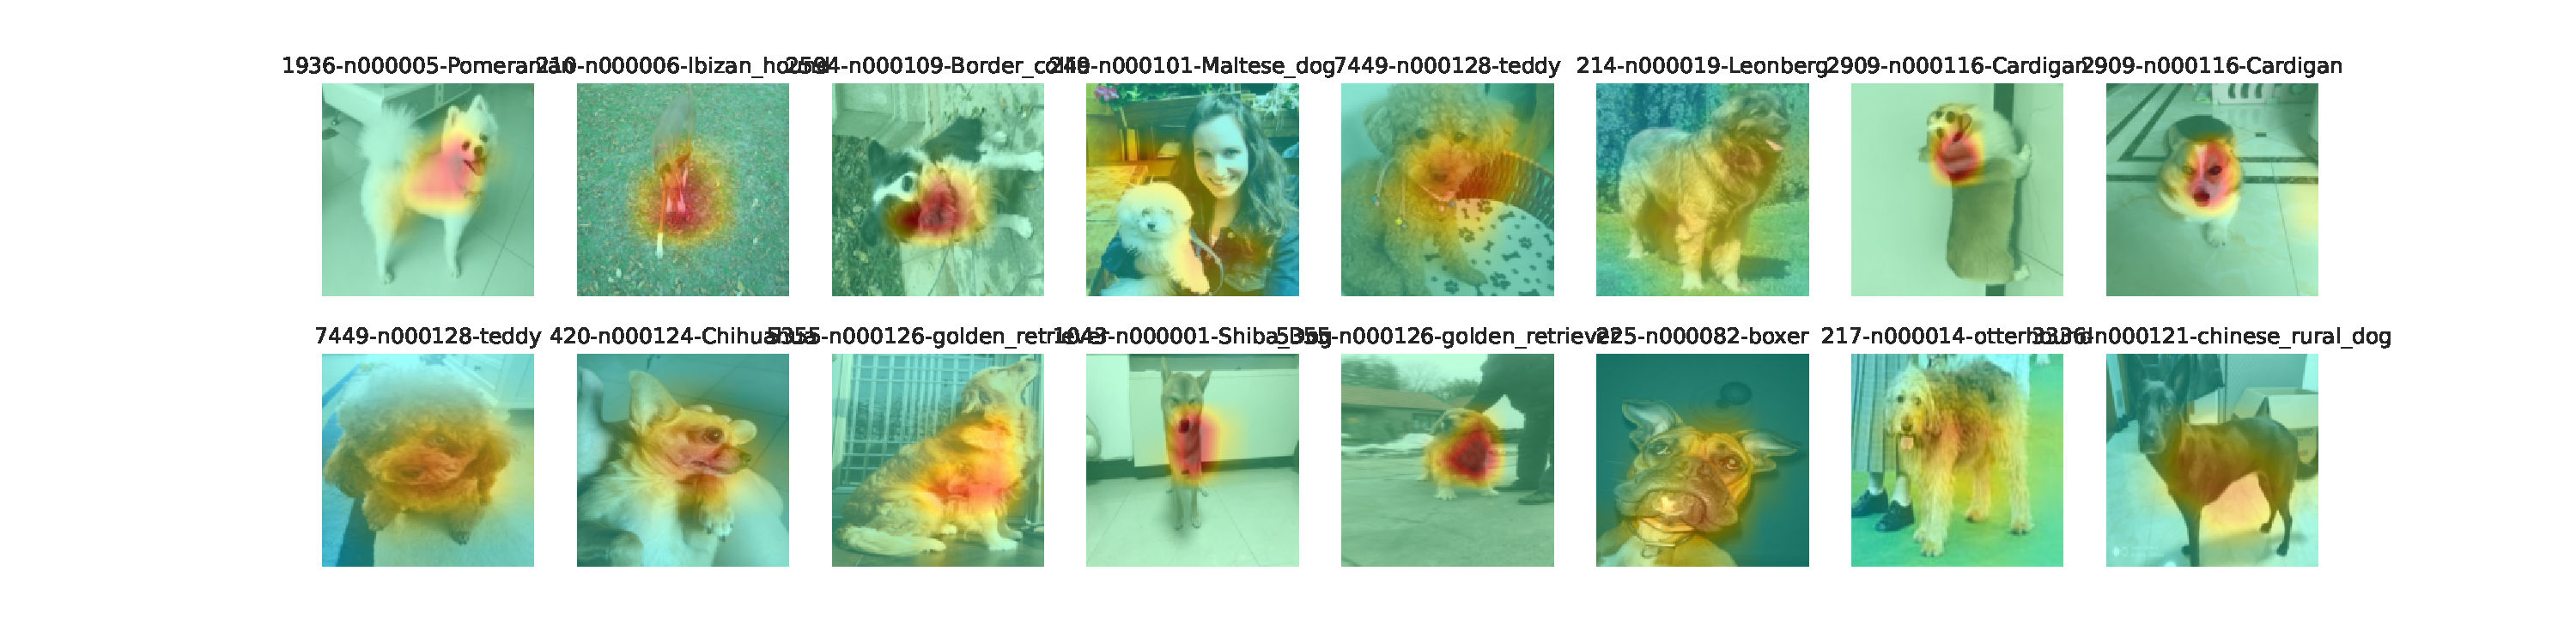
\includegraphics[width=\textwidth]{images/gpp_tsing_resnet50_proxy_3.pdf}
            \caption{With Proxy Attention}
        \end{subfigure}
        \caption{Comparison of attention maps generated by resnet50 trained with and without Proxy Attention on the tsing dataset}
    \end{figure}
    

    \begin{figure}[H]
        \begin{subfigure}[b]{1\textwidth}
            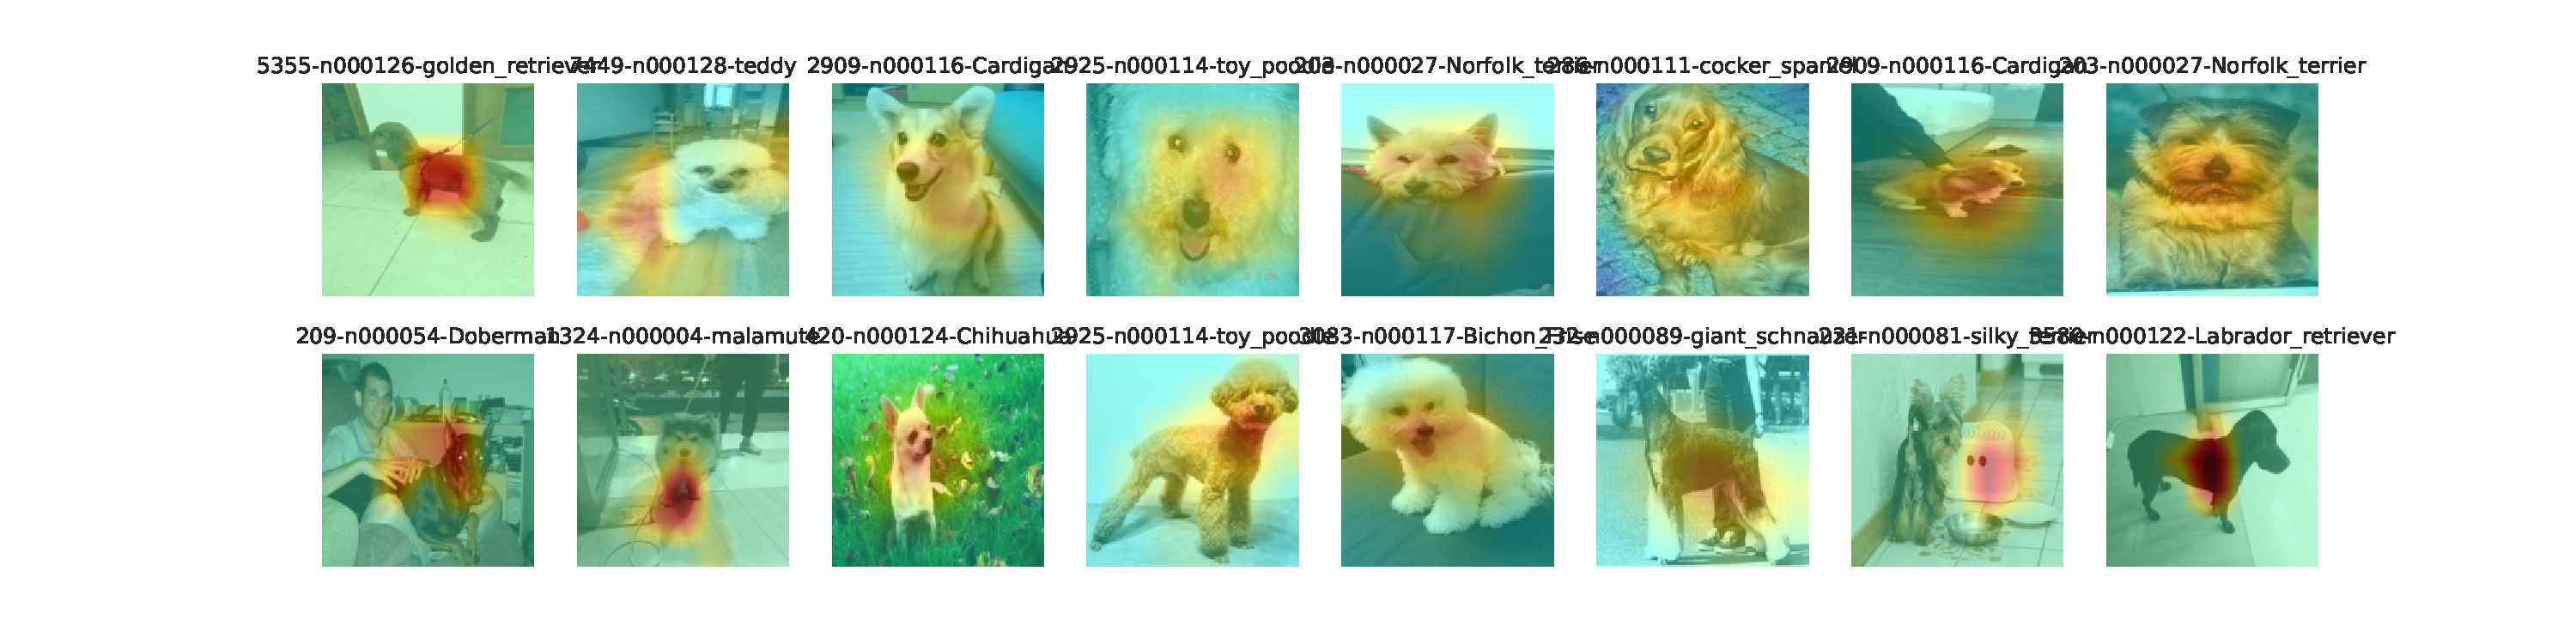
\includegraphics[width=\linewidth]{images/gpp_tsing_resnet50_noproxy_0.pdf}
            \caption{Without Proxy Attention}
        \end{subfigure}
        \begin{subfigure}[b]{1\textwidth}
            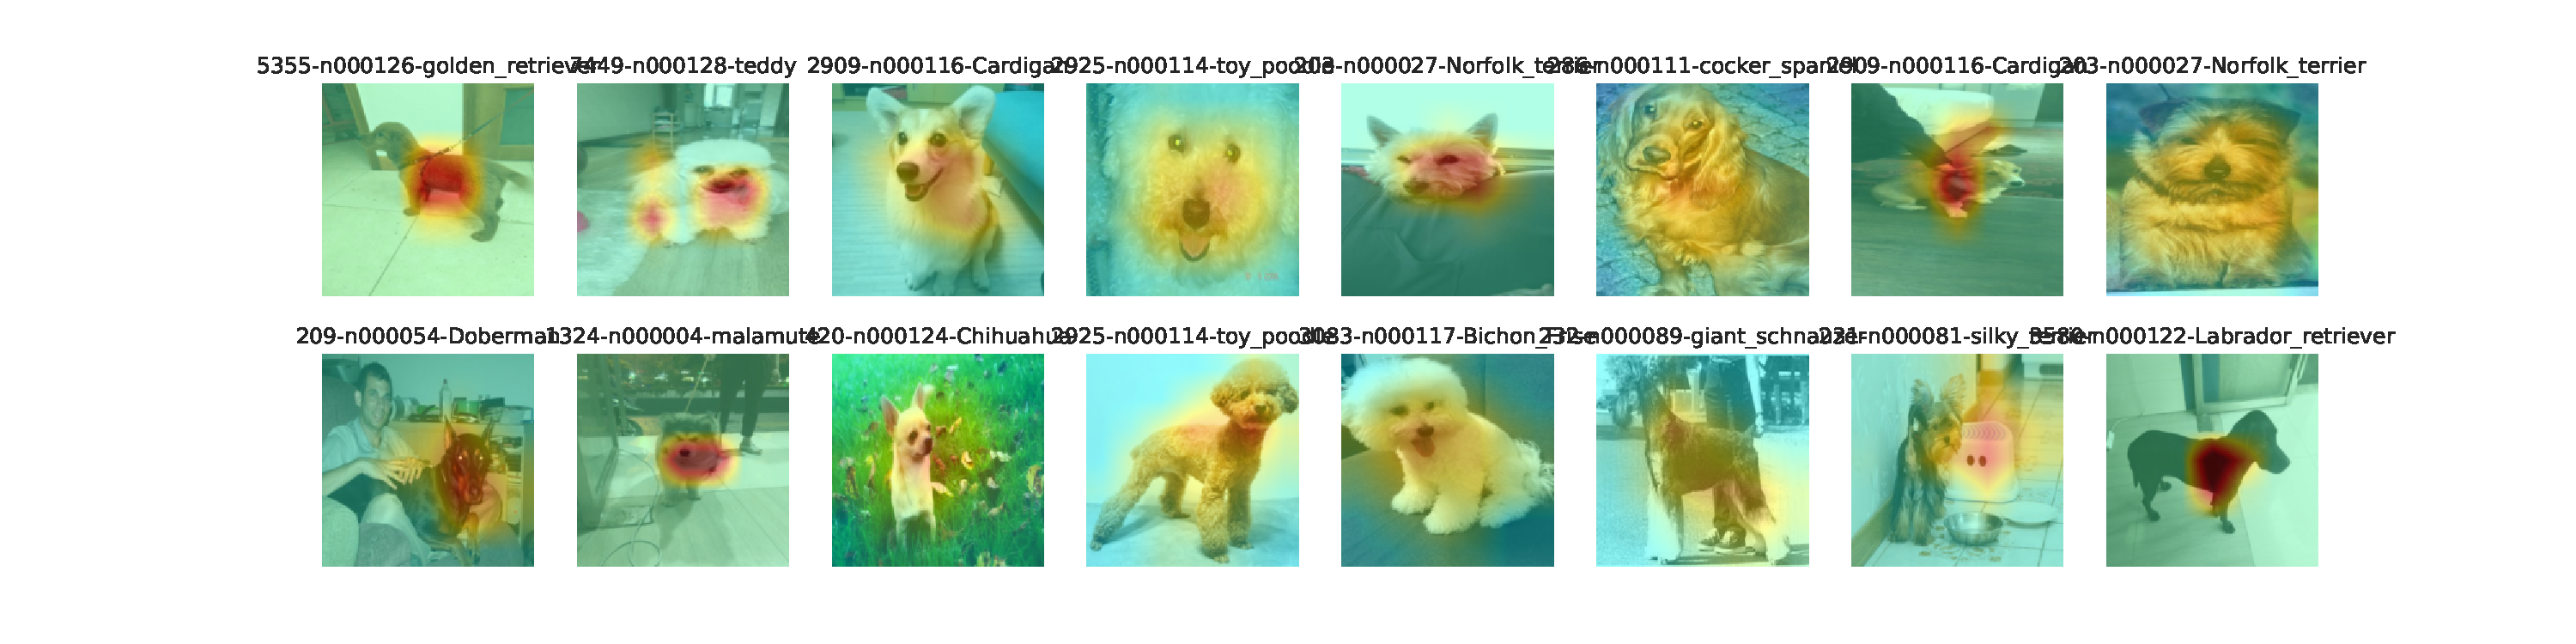
\includegraphics[width=\linewidth]{images/gpp_tsing_resnet50_proxy_0.pdf}
            \caption{With Proxy Attention}
        \end{subfigure}
        \caption{Comparison of attention maps generated by resnet50 trained with and without Proxy Attention on the tsing dataset}
    \end{figure}


\subsection{Tsinghua Dogs, ResNet18, EigenGradCAM}
    \begin{figure}[H]
        \begin{subfigure}[b]{1\textwidth}
            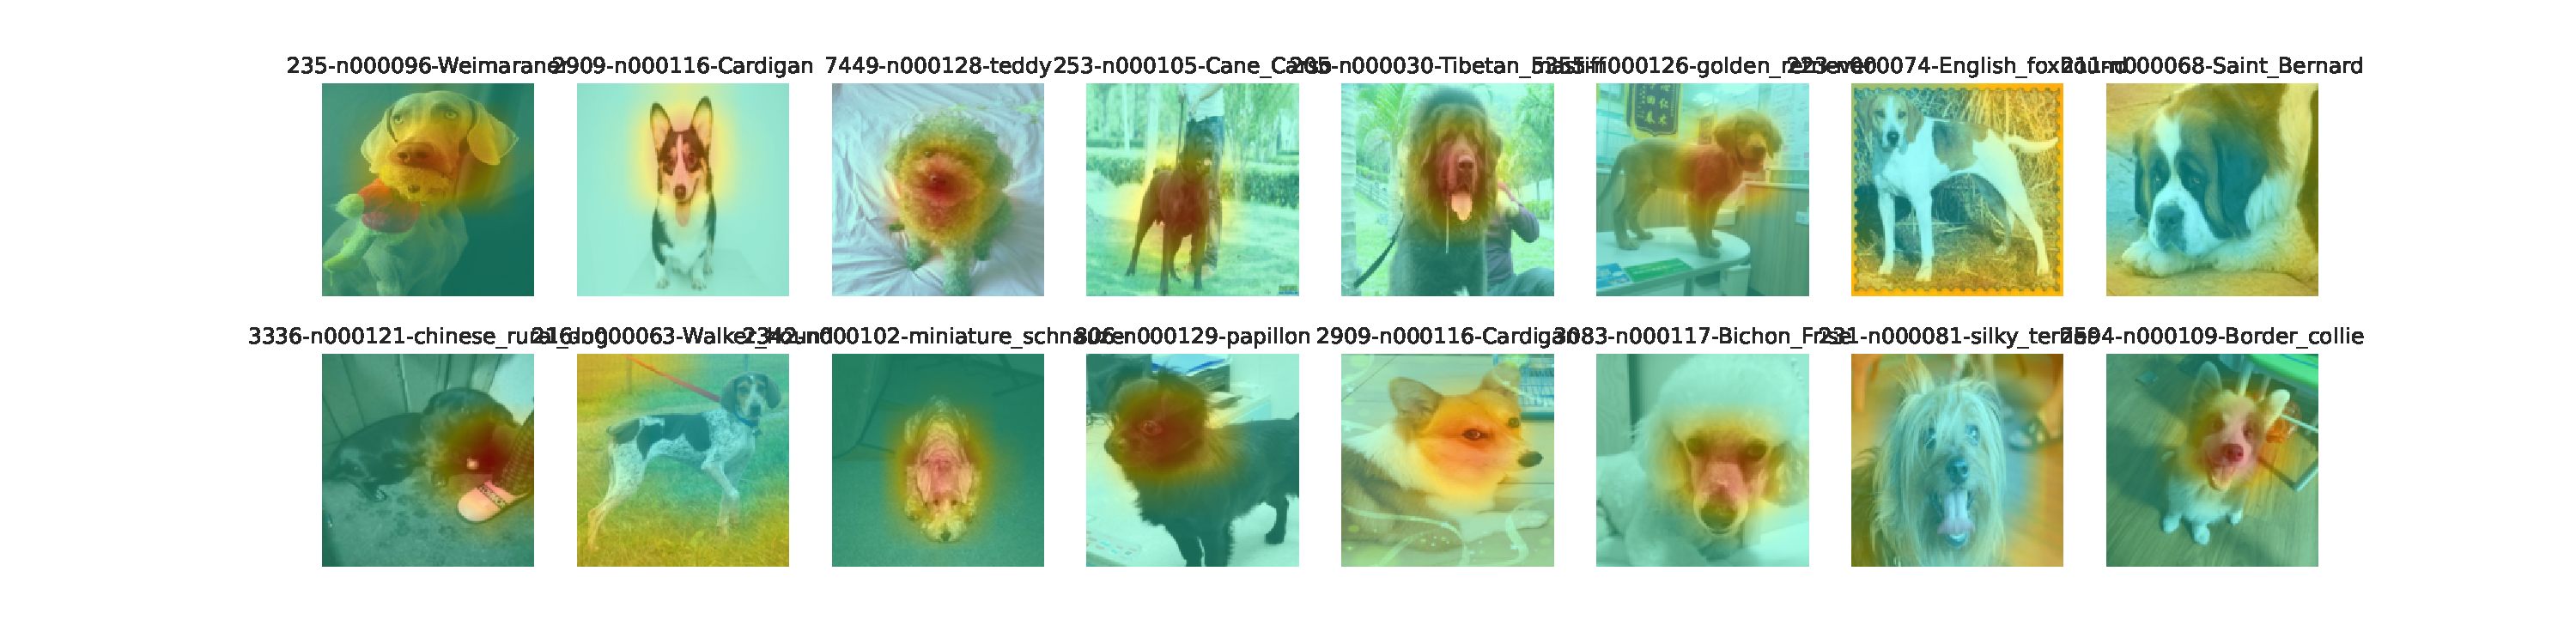
\includegraphics[width=\linewidth]{images/tsing_resnet18_noproxy_0.pdf}
            \caption{Without Proxy Attention}
        \end{subfigure}
        \begin{subfigure}[b]{1\textwidth}
            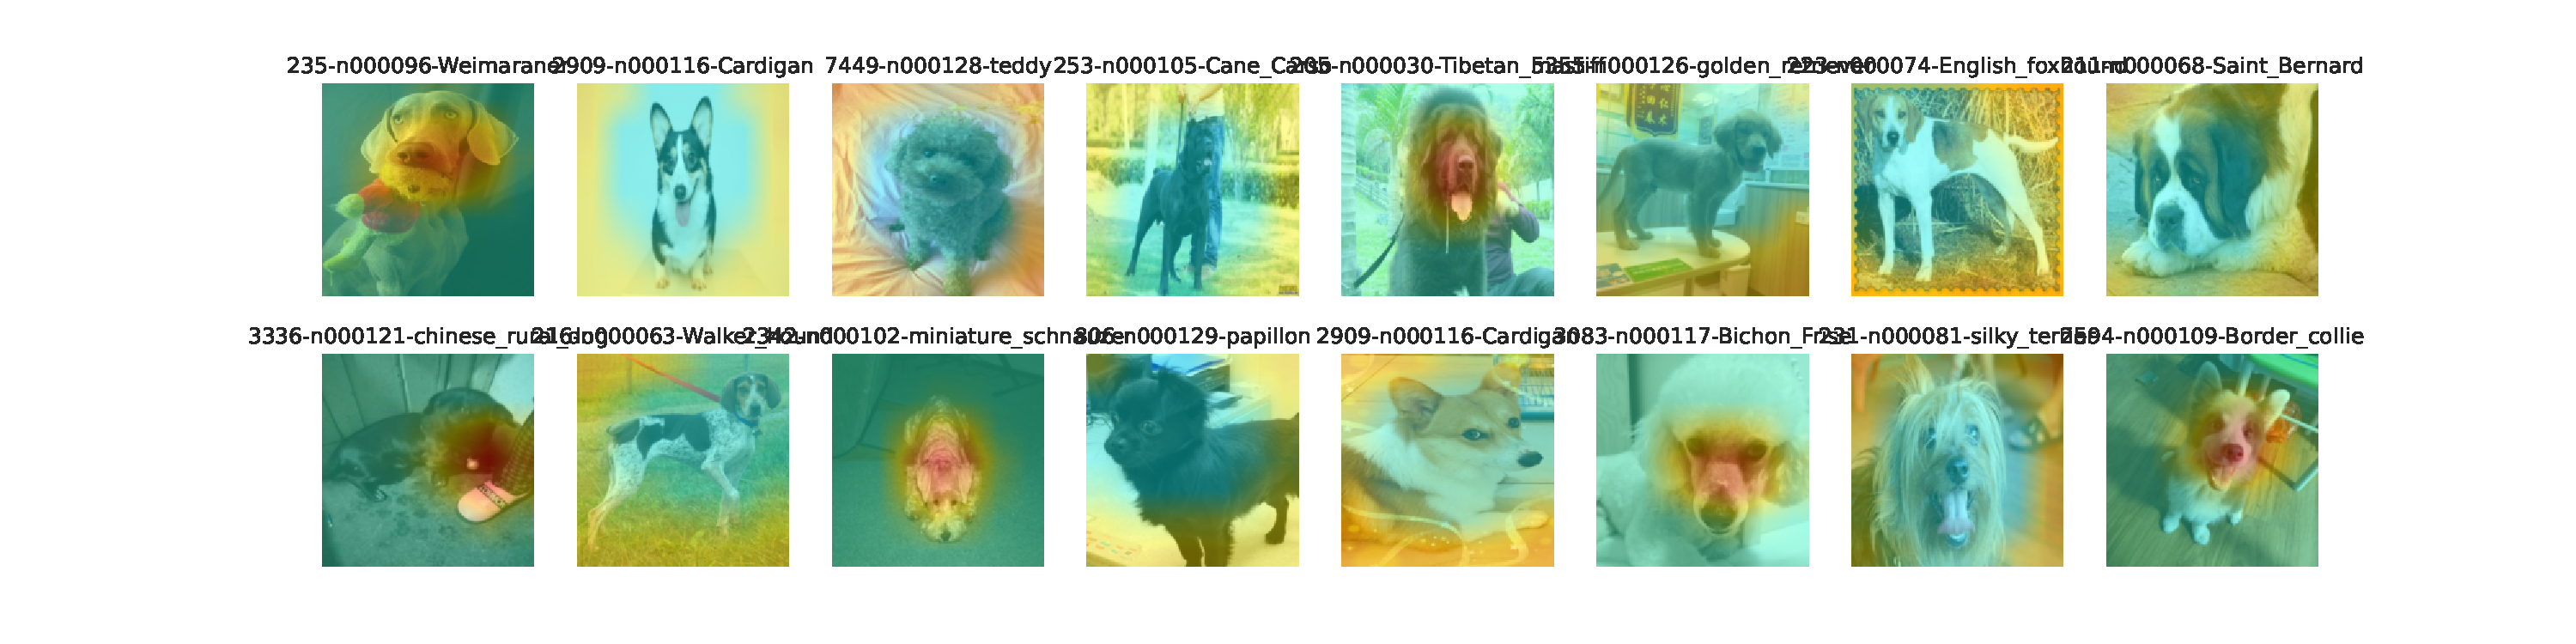
\includegraphics[width=\linewidth]{images/tsing_resnet18_proxy_0.pdf}
            \caption{With Proxy Attention}
        \end{subfigure}
        \caption{Comparison of attention maps generated by resnet18 trained with and without Proxy Attention on the tsing dataset}
    \end{figure}
    


